% !TEX root = ../main.tex
\title{Whole-brain multivariate deconvolution for multi-echo functional MRI}
\label{cha:multivariate}

\begin{framed}\noindent This chapter was published as
    \fullcite{Urunuela2022Wholebrainmultivariate}. DOI:
    \url{https://doi.org/10.1016/j.media.2023.103010}.
\end{framed}

This chapter proposes a novel hemodynamic deconvolution algorithm, multivariate
sparse paradigm free mapping (Mv-SPFM), that operates at the whole brain level
and adds spatial information via a mixed-norm regularization term over all
voxels. Additionally, \acrshort*{mvspfm} employs the stability selection
procedure that removes the need to select regularization parameters and also
lets us obtain an estimate of the true probability of having a neuronal-related
BOLD event at each voxel and time-point based on the area under the curve (AUC)
of the stability paths. Besides, its formulation is adapted for multi-echo fMRI
acquisitions (MvME-SPFM), which allows us to better isolate fluctuations of BOLD
origin on the basis of their linear dependence with the echo time (TE) and to
assign physiologically interpretable units (i.e., changes in the apparent
transverse relaxation $\Delta R_2^*$) to the resulting deconvolved events.
Remarkably, Mv-SPFM also achieves comparable performance when using a
conventional single-echo formulation. The MV-SPFM algorithm outperforms previous
hemodynamic deconvolution approaches, showing higher spatial and temporal
agreement with the activation maps and BOLD signals obtained with a standard
model-based linear regression approach. Furthermore, owing to the stability
selection, the proposed algorithm provides more reliable estimates of
neuronal-related activity for the study of the dynamics of brain activity when
no information about the timings of the BOLD events is available. This algorithm
is publicly available as part of the \textit{splora} Python package at
\url{https://github.com/ParadigmFreeMapping/splora}.

\section{Introduction}
\label{sec:multivariate_introduction}

Conventionally, the analysis of functional MRI (fMRI) data relies on available
information about the experimental paradigm to establish hypothesized models of
brain activity. However, this information can be inaccurate, incomplete or
unavailable in multiple scenarios such as resting-state, naturalistic paradigms
or clinical conditions. In these cases, blind estimates of neuronal-related
activity can be obtained with paradigm-free analysis methods such as hemodynamic
deconvolution. Yet, current formulations of the hemodynamic deconvolution
problem have three important limitations: 1) their efficacy strongly depends on
the appropriate selection of regularization parameters, 2) being univariate,
they do not take advantage of the information present across the brain, and 3)
they do not provide any measure of statistical certainty associated with each
detected event.

% Multi-echo fMRI for deconvolution. Adding spatial information. AUC: Wouldn't
% it be nice to have a probability of having an event at each time-point and for
% each voxel?
Despite the range of deconvolution methods that have been developed, few
capitalize on the various properties of fMRI data, such as the advantages of
multi-echo fMRI for denoising fMRI data
\citep{Bright2013Removingmotionphysiological, Kundu2017MultiechofMRI}, or the
use of tissue-based or parcellation-based information to improve the accuracy of
the estimates of neuronal activity. Recent exceptions include deconvolution
algorithms that incorporate a multivariate formulation to perform
spatio-temporal deconvolution
\citep{Bolton2019StructurallyInformedDeconvolution,Urunuela2021LowRankSparse,
Costantini2022Anisotropic4DFiltering,Cherkaoui2021Multivariatesemiblind}, thus
addressing the second limitation stated in the previous paragraph. In addition,
one deconvolution algorithm has been presented that exploits the
mono-exponential decay model of the multi-echo fMRI signal: multi-echo sparse
\acrlong*{pfm} (ME-SPFM) \citep{CaballeroGaudes2019deconvolutionalgorithmmulti}.
Furthermore, approaches have been developed to deal with the third limitation
stated above and estimate the likelihood of having a neuronal event at each
time-point and for each voxel by means of logistic regression
\citep{Bush2013Decodingneuralevents,Bush2015ImprovingprecisionfMRI} or Gaussian
mixture models \citep{Pidnebesna2019EstimatingSparseNeuronal}. However, wouldn't
it be desirable to have an algorithm that addresses all three limitations
mentioned above? Specifically, it would be beneficial to obtain a measure of the
probability of each voxel containing a neuronal event at each time-point using
regularized estimators, while also leveraging the spatio-temporal information
and physical properties of the fMRI signal for estimating the activity-inducing
signal.

% In this work...
This chapter proposes a novel approach for the hemodynamic deconvolution of fMRI
data that operates at the whole-brain level (i.e., multivariate formulation) to
incorporate spatial information through a mixed-norm regularization term.
Furthermore, this work proposes a stability selection procedure
\citep{Meinshausen2010Stabilityselection} that makes the estimation of the
neuronal activity more robust to the selection of the regularization parameters,
while providing the likelihood of having a neuronal-related event at each
time-point and for each voxel. Using multi-echo fMRI data acquired from 10
healthy subjects (16 datasets) this chapter demonstrates that the proposed
multivariate multi-echo \acrlong*{pfm} (MvME-SPFM) algorithm not only provides
more robust estimates of the neuronal activity, but also yields a measure of the
probability of each voxel containing a neuronal event at each time-point.
Moreover, MvME-SPFM returns quantitative estimates of $\Delta R_2^*$ in
interpretable units (s$^{-1}$), which is relevant for functional analysis across
different acquisition methods and field strengths. The chapter is structured as
follows: the multivariate signal model and the multivariate multi-echo PFM
algorithm are introduced in \cref{sec:multivariate_theory};
\cref{sec:multivariate_methods} describes the data used and the analysis
performed to evaluate this novel algorithm; the results of applying this new
algorithm on experimental fMRI data are presented and compared to the previous
PFM algorithms in \cref{sec:multivariate_results}; finally, the findings are
discussed in \cref{sec:multivariate_discussion}.

\section{Theory}
\label{sec:multivariate_theory}

\subsection{Signal Model for Whole-Brain Deconvolution}

\cref{cha:synthesis_analysis} introduced that the BOLD fMRI signal model of a
particular voxel can be written in matrix notation as:
\begin{equation}
    \mathbf{y} = \mathbf{H}\Delta\mathbf{s} + \mathbf{e}
    \label{eq:signal_model}
\end{equation}
where, assuming zero-boundary conditions, the variables $\mathbf{y}$, $\Delta
\mathbf{s}$, $\mathbf{e} \in \mathbb{R}^N$ are the voxel's time-series, the
activity-inducing signal changes and the noise term, respectively, and
$\mathbf{H} \in \mathbb{R}^{N \times N}$ is the Toeplitz convolution matrix
defined by the HRF
\citep{Gitelman2003Modelingregionalpsychophysiologic,Gaudes2013Paradigmfreemapping}.
Hereinafter in the chapter, the noise term is assumed to be an additive white
Gaussian noise (i.e., uncorrelated). Furthermore, the $\Delta \mathbf{s}$ can be
defined in a finer temporal resolution (i.e., increasing its dimension by a
factor $\alpha>1$ such that $\Delta \mathbf{s} \in \mathbb{R}^{\alpha N}$) so
that it can describe activity-inducing signal changes that are asynchronous to
the TR of the data. Though in such scenario, the convolution matrix becomes
non-Toeplitz (i.e. $\mathbf{H} \in \mathbb{R}^{N \times \alpha N}$)
\citep{Ciuciu2003Unsupervisedrobustnonparametric}.

The previous signal model is applicable for single-echo and multi-echo fMRI
data. In the particular case of multi-echo fMRI acquired with a gradient-echo
sequence, the voxel's time-series in terms of the signal percentage change has a
linear relationship with the echo time (TE) as $y(\mathrm{TE}_k,n) \approx
\Delta \rho(n) - \mathrm{TE}_k \Delta R_2^*(n)$,  
where $\Delta R_2^*(n)$ denotes the BOLD-like signal changes and $\Delta
\rho(n)$ corresponds to changes in the net magnetization, for instance due to
head motion \citep{Kundu2017MultiechofMRI}. The signal changes associated to
fluctuations in the net magnetization can be effectively reduced in
preprocessing, for example using multi-echo independent component analysis
\citep{Kundu2012DifferentiatingBOLDnon,CaballeroGaudes2019deconvolutionalgorithmmulti},
and are neglected hereinafter. Hence, considering that neuronal-related signal
changes $\Delta\mathbf{s}$ produce a change in $\Delta R_2^*$, the signal model
in Eq.\eqref{eq:signal_model} can be adapted to contain the signal acquired at
all $K$ echo-times (TE) via concatenation:

\begin{equation}
    \left[\begin{array}{c} \mathbf{y}_{1} \\
        \vdots \\
        \mathbf{y}_{K}
    \end{array}\right]
    =
    -\left[\begin{array}{c} \mathrm{TE}_{1} \mathbf{H} \\
        \vdots \\
        \mathrm{TE}_{K} \mathbf{H}
    \end{array}\right]
    \Delta \mathbf{s},
\label{eq:univariate_multi-echo_model}
\end{equation}
which can be simplified into $\bar{\mathbf{y}}=-\overline{\mathbf{H}} \Delta
\mathbf{s}$, where $\bar{\mathbf{y}} \in \mathbb{R}^{KN}$, $\Delta \mathbf{s}
\in \mathbb{R}^{N}$ and $\overline{\mathbf{H}} \in \mathbb{R}^{KN \times N}$. 

Assuming that the shape of the hemodynamic response can be similarly modeled
across all brain voxels, the previous voxel-wise (i.e., univariate) model in
Eq.\eqref{eq:univariate_multi-echo_model} can be extended straightforwardly to a
multivariate formulation that considers all the voxels $V$ of the brain:

\begin{equation}
    \begin{bmatrix}
        \mathbf{y}_{1,1} & \cdots & \mathbf{y}_{1,V} \\
        \vdots & \ddots & \vdots \\
        \mathbf{y}_{K,1} & \cdots & \mathbf{y}_{K,V}
    \end{bmatrix}
    =
    -
    \begin{bmatrix}
        \mathrm{TE}_{1} \mathbf{H} \\
        \vdots \\
        \mathrm{TE}_{K} \mathbf{H}
    \end{bmatrix}
    \begin{bmatrix}
        \Delta \mathbf{s}_1 & \cdots & \Delta \mathbf{s}_V \\
    \end{bmatrix},
\label{eq:multivariate_multi-echo_model}
\end{equation}
which can be simplified into $\bar{\mathbf{Y}} = - \bar{\mathbf{H}} \Delta
\mathbf{S}$, where $\bar{\mathbf{Y}} \in \mathbb{R}^{KN \times V}$,
$\bar{\mathbf{H}} \in \mathbb{R}^{KN \times N}$ and $\Delta\mathbf{S} \in
\mathbb{R}^{N \times V}$.

\section{Solving the Optimization Problem for Whole-Brain Deconvolution}

As described in \cref{cha:synthesis_analysis}, an estimate of the activity that
induces the BOLD response $\hat{\mathbf{s}}$ can be obtained by solving an
ordinary least-squares problem such as:
\begin{equation}
    \Delta \hat{\mathbf{s}} = \arg \min_{\mathbf{s}} \frac{1}{2}
    \| \bar{\mathbf{y}} - \bar{\mathbf{H}} \Delta \mathbf{s} \|_2^2
    + \lambda \| \Delta \mathbf{s} \|_1,
\label{eq:univariate_multi-echo_inverse_problem}
\end{equation}
where $\lambda$ is the regularization parameter that regulates the level of
sparsity of the estimates given the $\ell_1$-norm, which is defined as $\|
\Delta \mathbf{s} \|_1 = \Sigma_{n=1}^{N} | \Delta \mathbf{s}_n |$.

The inverse problem in Eq.\eqref{eq:univariate_multi-echo_inverse_problem} can
be directly adapted to be solved at the whole-brain using the multivariate
formulation in Eq.\eqref{eq:multivariate_multi-echo_model}. More interestingly
though, solving the inverse problem at the whole-brain level opens up many
possibilities in the form of additional regularization terms to take advantage
of the spatial information for an informed estimation of the activity-inducing
signal $\Delta\hat{\mathbf{S}}$. For instance, mixed-norms in the form of
$\ell_{p,q}$ can be employed to separate coefficients into groups that are blind
to each other, while the coefficients within a group are treated together
\citep{Kowalski2009Sparseregressionusing}. Hence, regularization terms based on
mixed-norms can promote spatio-temporal structures that are observed in fMRI
signals. 

Here, an $\ell_{2,1} + \ell_1$ mixed-norm regularization term
\citep{Gramfort2011FunctionalBrainImaging} is added to the multivariate convex
problem to promote the co-activation of the activity-inducing signal
$\Delta\hat{\mathbf{S}}$ considering the coefficients of the voxels of the brain
($V$) at time $n$ as one group:

\begin{equation}
    \Delta \hat{\mathbf{S}} = \arg \min_{\mathbf{S}} \frac{1}{2}
    \| \bar{\mathbf{Y}} - \bar{\mathbf{H}} \Delta \mathbf{S} \|_2^2
    + \lambda \rho \| \Delta \mathbf{S} \|_1
    + \lambda (1 - \rho) \| \Delta \mathbf{S} \|_{2,1},
    \label{eq:multivariate_multi-echo_inverse_problem}
\end{equation}
where $\ell_{2,1}$-norm is defined as $\| \Delta \mathbf{S} \|_{2,1} =
\Sigma_{n=1}^{N} \sqrt{ \Sigma_{v=1}^{V} \Delta \mathbf{S}_{n,v}^2} $, and
$0<\rho<1$ is a parameter that controls the tradeoff between the sparsity
introduced by the $\ell_1$-norm and the grouping of voxels promoted by the
$\ell_{2,1}$-norm so that the estimation of one voxel coefficient at time $n$ is
influenced by the estimates of the rest of the brain voxels at the same time.
Note that when $\rho=1$ Eq.~\eqref{eq:multivariate_multi-echo_inverse_problem}
is the whole-brain equivalent of
Eq.~\eqref{eq:univariate_multi-echo_inverse_problem}. Additionally, it is worth
noting that mixed-norm regularization, such as group LASSO, has been previously
used in MEG/EEG studies \citep{Gramfort2011FunctionalBrainImaging}. However, in
those cases, the spatial and temporal dimensions were swapped compared to
Eq.~\eqref{eq:multivariate_multi-echo_inverse_problem}.On the other hand, the
regularization parameter $\lambda$ can be adapted voxel-wise in order to account
for differences in the signal-to-noise ratio across voxels. Consequently, the
multivariate deconvolution problem can be written as:

\begin{equation}
    \Delta \hat{\mathbf{S}} = \arg \min_{\mathbf{S}} \frac{1}{2}
    \| \bar{\mathbf{Y}} - \bar{\mathbf{H}} \Delta \mathbf{S} \|_2^2
    + \rho \| \mathbf{D} \Delta \mathbf{S} \|_1
    + (1 - \rho) \| \mathbf{D} \Delta \mathbf{S} \|_{2,1},
    \label{eq:multivariate_multi-echo_inverse_problem2}
\end{equation}
where $\mathbf{D} = \text{diag}\left(\lambda_1, \dots, \lambda_V \right) \in
\mathbb{R}^{V \times V}$ is a diagonal matrix with the voxel-specific values of
$\lambda$. In practice, a criterion must be used to select the voxel-specific
$\lambda$s. Instead, the use of stability selection to avoid this critical
choice is proposed (see \cref{sec:multivariate_stability_selection}). 

Therefore, given the convex nature of the inverse problem in
Eq.~\eqref{eq:multivariate_multi-echo_inverse_problem2}, estimates of $\Delta
\hat{\mathbf{S}}$ can be calculated using the fast iterative
shrinkage-thresholding algorithm (FISTA) \citep{Beck2009FastIterativeShrinkage}
with the following proximity operator for $\ell_1 + \ell_{2,1}$:

\begin{equation}
    S_{n,v} = \frac{Z_{n,v}}{|Z_{n,v}|} \left( |Z_{n,v} - \lambda_v \rho \right)^+ \left( 1 - \frac{\lambda_v (1 - \rho)}{\sqrt{ \sum_v \left( |Z_{n,v}| - \lambda_v \rho \right)^{+^2} }} \right)^+,
    \label{eq:multivariate_multi-echo_proximal_operator}
\end{equation}
where $\Delta \mathbf{S} = \text{prox}_{\lambda \left(\rho \| \cdot \|_1 +
\left( 1 - \rho \right) \| \cdot \|_{2,1} \right)}\left(\mathbf{Z} \right) \in
\mathbb{R}^{N \times V}$, $\left( x \right)^+ = \max \left( x,0 \right)$ for $x
\in \mathbb{R}$, and $\frac{0}{0}=0$ by convention.

\section{Methods}
\label{sec:multivariate_methods}
\subsection{fMRI Data Acquisition and Preprocessing}

The evaluation of the proposed MvME-SPFM was performed on ME-fMRI data acquired
in 10 subjects using a multi-task rapid event-related paradigm. Six subjects
performed two functional runs, the other 4 subjects only performed 1 run due to
scanning time constraints (i.e., a total of 16 datasets). All participants gave
informed consent in compliance with the NIH Combined Neuroscience International
Review Board-approved protocol 93-M-1070 in Bethesda, MD. A thorough description
of the MRI acquisition protocols and experimental tasks in the experimental
design can be found in \citep{GonzalezCastillo2016Evaluationmultiecho}, only
those details that are relevant to this analysis are given here.

MRI data was acquired on a General Electric 3T 750 MRI scanner with a 32-channel
receive-only head coil (General Electric, Waukesha, WI). Functional scans were
acquired with a ME gradient-recalled echoplanar imaging (GRE-EPI) sequence (flip
angle = $70^\circ$ for 9 subjects, flip angle = $60^\circ$ for 1 subject, TEs =
16.3/32.2/48.1 ms, TR = 2 s, 30 axial slices, slice thickness = 4 mm, in-plane
resolution = $3\times3$ mm$^2$, FOV 192 mm, acceleration factor 2, number of
acquisitions = 220). Functional data was acquired with ascending sequential
slice acquisitions, except in one subject where the acquisitions were
interleaved. In addition, high resolution T1-weighted MPRAGE and proton density
images were acquired per subject for anatomical alignment and visualization
purposes (176 axial slices, voxel size = $1\times1\times1$ mm$^3$, image matrix
= $256\times256$).

Each run of data acquisition consisted of 6 trials with 5 different tasks each:
biological motion observation (BMOT), finger tapping (FTAP), passive viewing of
houses (HOUS), listening to music (MUSI), and sentence reading (READ). The
reader is referred to that paper for details on the preprocessing steps, and
comparison with alternative single-echo models for deconvolution. This data had
previously been employed, preprocessed and ME-ICA denoised for the evaluation of
the ME-SPFM algorithm in \citep{CaballeroGaudes2019deconvolutionalgorithmmulti}.

\subsection{Stability Selection of the Regularization Parameter $\lambda$}
\label{sec:multivariate_stability_selection}

The choice of the regularization parameter $\lambda$ is crucial to obtain
accurate estimates of $\Delta \hat{\mathbf{S}}$. Although the value of $\lambda$
of each voxel could be fixed ad-hoc, previous work has opted for the use of
model selection criteria, such as the Bayesian Information Criterion (BIC), on
the regularization path \citep{CaballeroGaudes2019deconvolutionalgorithmmulti},
computed by means of the least angle regression (LARS) algorithm
\citep{Efron2004Leastangleregression}. Even though the use of BIC performed well
for ME-SPFM \citep{CaballeroGaudes2019deconvolutionalgorithmmulti} and its
single-echo counterpart (SPFM) \citep{Gaudes2013Paradigmfreemapping}, due to its
high specificity, it can be problematic for certain voxels where the BIC curve
might present multiple local minima or even fail to present a clear minima for
the evaluated range of $\lambda$.

This chapter proposes a more robust procedure to address this shortcoming 
for selecting $\lambda$ with the usage of the stability selection method
\citep{Meinshausen2010Stabilityselection} described in \cref{cha:stability}. 
Moreover, the stability selection procedure presented here yields the probability 
to have a non-zero coefficient in the activity-inducing signal at each time-point. 
Specifically, our implementation of the stability selection procedure generates $T=30$ 
surrogates of each voxel timecourse by randomly subsampling 60\% of the time-points (a 
more computationally expensive version was also tested with $T=100$ surrogates that
yielded very similar results). The convolution matrix $\mathbf{H}$ is subsampled
accordingly. The surrogate data is then analyzed with the inverse problem in
Eq.~\eqref{eq:multivariate_multi-echo_inverse_problem} for a voxel-specific
range of $\lambda$ values using the fast iterative shrinkage thresholding
algorithm (FISTA). Here, 30 values of $\lambda$ are spaced logarithmically
between 5\% and 95\% of the voxel-specific maximum $\lambda$ possible to more
accurately sample the lower range. Then, the ratio (probability) of surrogates
where the estimated coefficient at each time-point is non-zero is calculated for
each time-point and value of $\lambda$.  As illustrated in
\cref{fig:reg_and_stab_paths}, these probabilities build the so-called stability
paths, which resemble the well-known regularization paths of conventional
regularized estimators (e.g., LASSO, Ridge Regression) that plot the amplitude
of the coefficients for each $\lambda$. 

Unlike the original stability selection procedure, which sets a given
probability threshold to select the final set of non-zero coefficients
\citep{Meinshausen2010Stabilityselection}, the area under the curve (AUC) of the
stability path of each time-point is calculated as an index of confidence of
having a non-zero coefficient across the evaluated range of $\lambda$. As a
result, the \acrshort*{auc} timecourse provides a measure of the probability of
having neuronal-related activity at each time-point and voxel. Next, the AUC
time-series are thresholded according to the histogram of AUC values in a region
of non-interest (hereinafter, denoted as the null AUC histogram) to yield a
sparse representation of the signal. Alternatively, a null distribution of AUC
values could be generated from surrogate data
\citep{Liegeois2021Interpretingnullmodels}. Accordingly, when employing
stability selection, the individual voxels' estimates might not be equivalent to
the voxels' estimates in any single one of the whole-brain models that can be
formulated with a given value of $\lambda$ in
Eq.\eqref{eq:multivariate_multi-echo_inverse_problem} or $\mathbf{D}$ in
Eq.~\eqref{eq:multivariate_multi-echo_inverse_problem2}), but are rather
obtained by computing area-under-the-curve (AUC) values for neuronal-related
events.

Finally, a fitting step is applied to each voxel by defining a reduced
convolution model with the selected non-zero coefficients and fitting it by
means of a conventional orthogonal least squares estimator. This step reduces
the bias towards zero imposed by the sparsity-promoting regularization terms,
and thus obtains more realistic estimates of the neuronal-related signal (here,
in terms of $\Delta R_2^*$)
\citep{CaballeroGaudes2019deconvolutionalgorithmmulti}.

% Regularization path and stability path figure
\begin{figure}[t!]
    \centerline{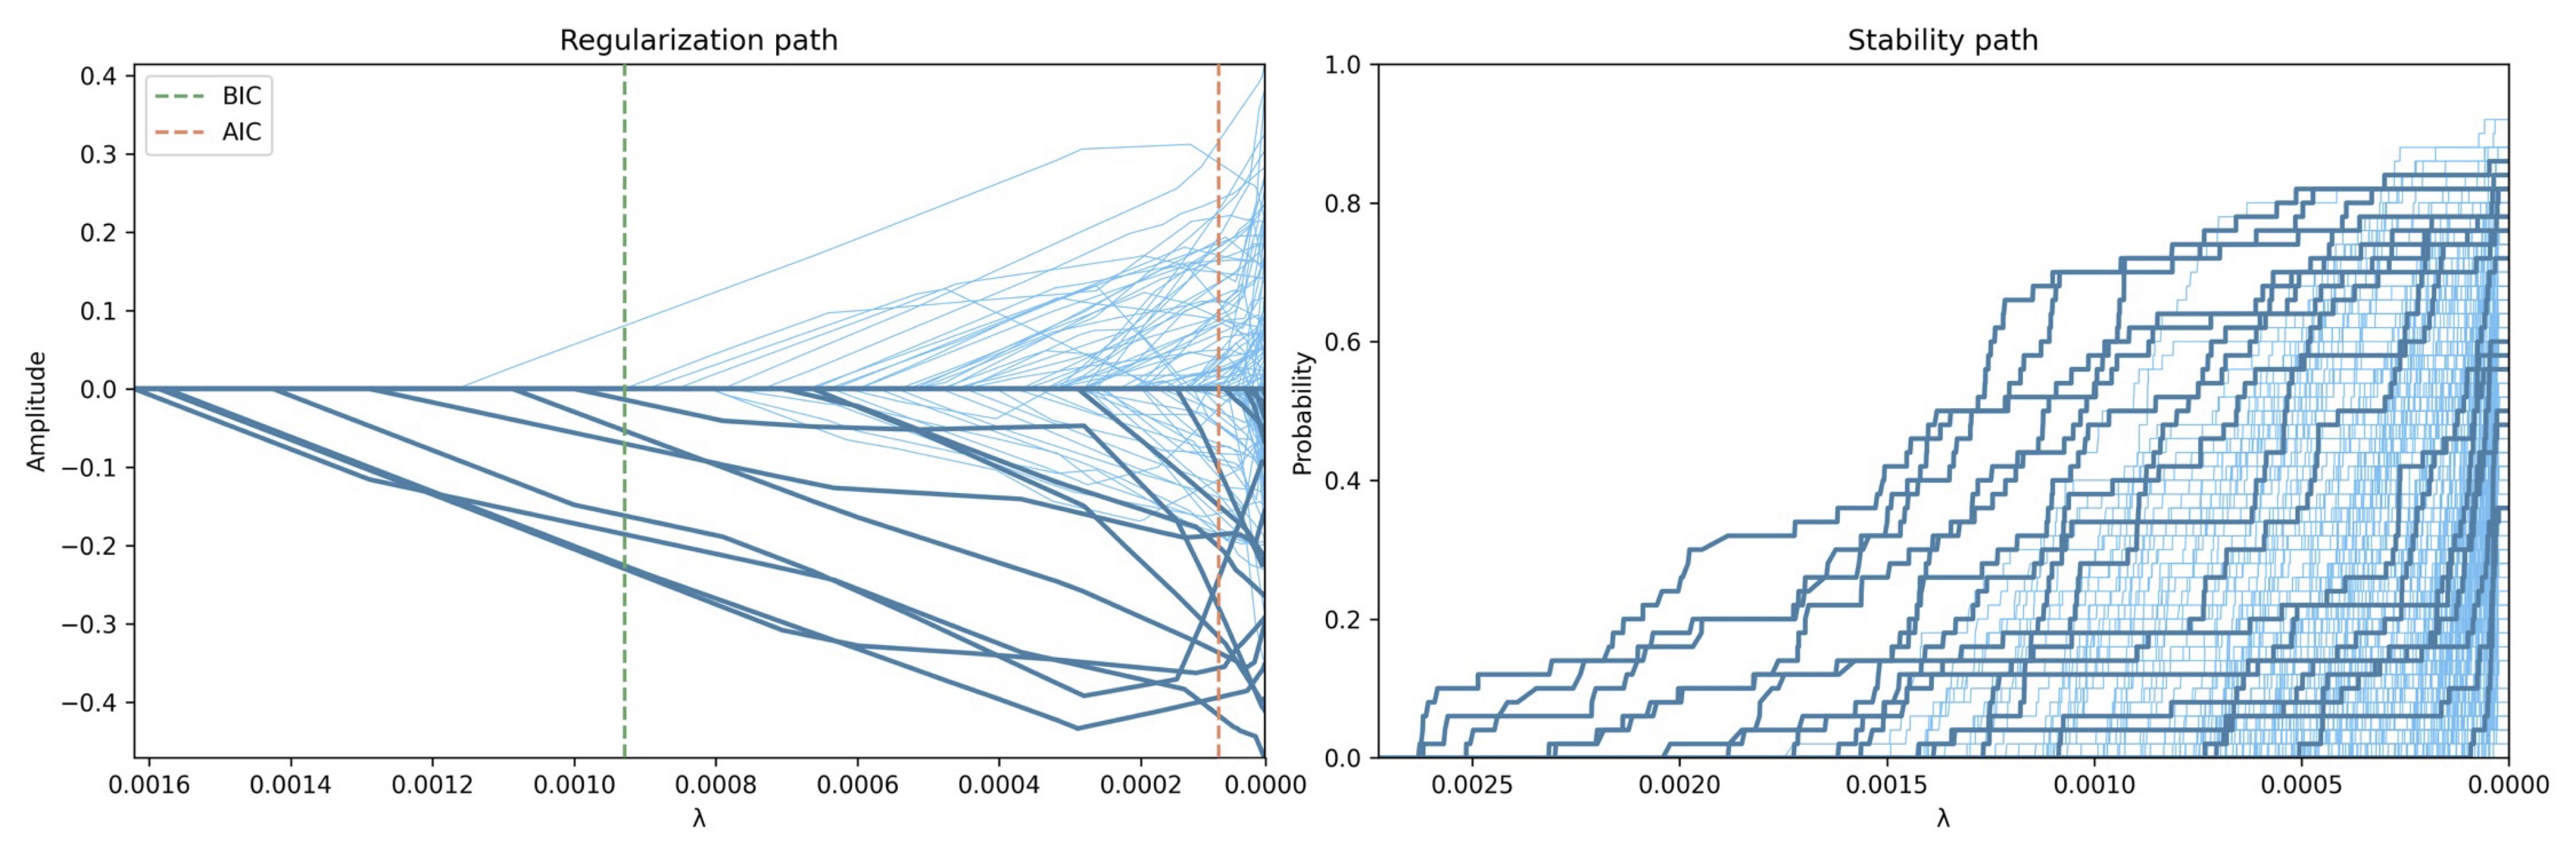
\includegraphics[width=\textwidth]{figures/multivariate/reg_and_stab_paths.jpg}}
    \caption{Example of the regularization path and the stability path for a
    voxel timeseries with $\rho=1$. On the left, the regularization path shows
    the amplitude of each coefficient estimate $\Delta \hat{\mathbf{S}}$ (one
    per TR). At first, all the coefficients are zero and successively they
    become non-zero as $\lambda$ decreases towards zero, which corresponds to
    the orthogonal least squares solution (i.e., no regularization). On the
    right, the corresponding stability path plots the probablity that each
    coefficient estimate (i.e., each TR) is non-zero for each value of $\lambda$
    based on the stability selection procedure. Note that both paths can have a
    different maximum value of $\lambda$ given the subsampling step in the
    stability selection. Lines in the stability path correspond to different TRs
    of a single voxel. The darker lines denote the coefficient estimates
    corresponding to the TRs during the task-related events.}
\label{fig:reg_and_stab_paths}
\end{figure}

\subsection{Balancing the Spatial Regularization}

The $\ell_{2,1}$-norm regularization term in
Eq.~\eqref{eq:multivariate_multi-echo_inverse_problem} promotes structured
spatio-temporal sparsity in the sense that the estimates of all brain voxels at
a given time-point are treated as a group and this term forms a constraint on
the number of groups with at least one non-zero estimate to model the data.
Assuming that $\rho=0$, either the value of all the voxel estimates at one time
point can be non-zero or all of them are nulled. Hence, this regularization term
considers spatial information from all brain voxels for the deconvolution since
the value of a given voxel coefficient also depends on the rest of the voxels. 

To illustrate the effect of the corresponding regularization parameter $\rho$,
this chapter solves the multivariate regularization problem in
Eq.~\eqref{eq:multivariate_multi-echo_inverse_problem} using stability selection
for $\rho=1$, $\rho=0.5$ and $\rho=0$.; i.e., applying the sparsity-promoting
$\ell_1$-norm only, equally weighting the sparsity and spatial regularizations,
and employing the $\ell_{2,1}$-norm spatial regularization only, respectively.

\subsection{Comparison with Conventional Timing-Based GLM Analyses}

To evaluate how the multivariate formulation combined with stability selection
improves the accuracy of the estimates of $\Delta \hat{\mathbf{S}}$ compared
with its univariate counterpart ME-SPFM using the BIC for voxel-wise selection
of $\lambda$ \citep{CaballeroGaudes2019deconvolutionalgorithmmulti}, the spatial
sensitivity, specificity and overlap (using a Dice coefficient metric) of the
MvME-SPFM activation maps were calculated using the trial-level GLM-based
activation maps ($p \leq 0.05$) as the ground truth. These analyses were
computed with the independently modulated (IM) option of the 3dDeconvolve
program in AFNI that implements an orthogonal least squares estimation for each
trial, thus also assuming uncorrelated noise as in our model. Single trial GLM
maps (GLM-IM) were obtained from the optimally combined and ME-ICA denoised
data, and only negative $\Delta R_2^*$ (i.e., $\Delta \hat{\mathbf{S}} < 0$ that
generate a positive BOLD response) were considered for the computation of the
Dice coefficients. 

For the MvME-SPFM, the following two strategies for thresholding the AUC
timeseries were considered in order to define the corresponding activation maps:
\begin{itemize}
    \item \textbf{Static thresholding {(ST)}:} The estimates of $\Delta
    \hat{\mathbf{S}}$ obtained with the novel MvME-SPFM technique that utilizes
    stability selection, where the AUC threshold was chosen as the 95th
    percentile of the histogram of AUC in deep white matter voxels (i.e., a
    fixed, static threshold), which were labeled after tissue segmentation of
    the T1-weighted anatomical MRI using \textit{3dSeg} in AFNI, and eroding 4
    voxels of the resulting white matter tissue mask at anatomical resolution. 
    \item \textbf{Time-dependent thresholding {(TD)}:} The estimates of $\Delta
    \hat{\mathbf{S}}$ obtained with the novel MvME-SPFM technique with stability
    selection, where the AUC threshold varies temporally according to the 95th
    percentile of the null histogram of AUC at each time-point. This
    implementation was based on the hypothesis that a time-dependent threshold
    would be able to better control for widespread spurious deconvolved changes
    in $\Delta \hat{\mathbf{S}}$, for instance due to head motion or deep
    breaths. 
\end{itemize}

Note the ST and TD thresholding strategies can be applied in the analysis of
single-echo and multi-echo fMRI data. 

\subsection{Comparison with Another State-of-the-Art Multivariate Deconvolution Method}

In order to evaluate how the MvME-SPFM algorithm compares with another
state-of-the-art multivariate deconvolution method, Hemolearn
\citep{Cherkaoui2021Multivariatesemiblind} was chosen, a recently proposed
multivariate semi-blind deconvolution method that can estimate the HRF and the
neuronal signal in a paradigm-free setting and that has been shown to faithfully
capture intrinsic functional connectivity networks at the subject level. This
technique introduces a low-rank constraint to learn both $K$ temporal atoms
(with $K \ll P$ ) and their corresponding spatial maps, which encode various
functional networks, each of them with their specific neural activation profile.
Hence, HemoLearn models the brain activity as a linear combination between the
neural activations $Z = \left( z_k \right)_{k=1}^K \in \mathbb{R}^{K \times T}$
and the spatial patterns $U = \left( u_k \right)_{k=1}^K \in \mathbb{R}^{K
\times P}$, where $T$ is the total number of TRs in the data and $P$ is the
number of voxels. The BOLD fMRI signal model is then given by the convolution between
an estimated regional HRF and the activation as:

\begin{equation}
    \mathbf{Y} = \left( \sum_{m=1}^M \mathbf{H_m} \right) * \left( \sum_{k=1}^K \mathbf{u_k}^T \mathbf{z_k} \right) + \mathbf{E}
\end{equation}

Thus, the minimization problem proposed by HemoLearn can be described as:

\begin{equation}
    \arg \min_{\mathbf{U}, \mathbf{Z}} = \frac{1}{2} \| \mathbf{Y} - \left( \sum_{m=1}^M \mathbf{H_m} \right) * \left( \sum_{k=1}^K \mathbf{u_k}^T \mathbf{z_k} \right) \|_F^2 + \lambda \sum_{k=1}^K \| \nabla \mathbf{z_k} \|_1
\end{equation}

The practical implementation of Hemolearn --which is available at
\url{https://hemolearn.github.io/}-- requires the specification of the number of
components to be estimated, which has no standard procedure to be determined.
Here, the analysis was performed with a range of components from 5 to 40. With
the aim of making the comparison as fair as possible, the component that
maximized the correlation between the estimated activity map and the
session-level GLM-based activation map was selected for each condition in the
task. The selected component time-series were compared with the corresponding
$\Delta \hat{\mathbf{S}}$ obtained with MvME-SPFM using stability selection and
the time-dependent thresholding (TD), and the selected component activity maps
with the corresponding trial-level MvME-SPFM activity maps obtained with the
same thresholding strategy.

\section{Results}
\label{sec:multivariate_results}

The output of deconvolution algorithms such as ME-SPFM and the proposed
MvME-SPFM is a 4D dataset that matches the dimensions (both spatial and
temporal) of the input data, i.e., it is a movie of the estimated $\Delta R_2^*$
maps. In addition, the use of stability selection generates the area under the
curve (AUC) 4D output dataset, which indicates the probability of having a
neuronal-related event at each time-point for every voxel in the brain. 

\cref{fig:auc} depicts the area under the curve (AUC) time-series and maps
obtained with stability selection for $\rho=0.5$ in representative voxels of
each task in the paradigm (indicated with a cross in the maps), where the AUC
maps correspond to single time-points signaled by the blue arrows. The AUC
time-series of the ST and TD thresholding approaches are shown on top of the
original AUC time-series. The AUC maps depict spatial patterns of $\Delta R_2^*$
where regions that are typically involved in the tasks show higher probabilities
of having neuronal-related activity compared with other brain regions.

\begin{figure}[ht!]
    \centerline{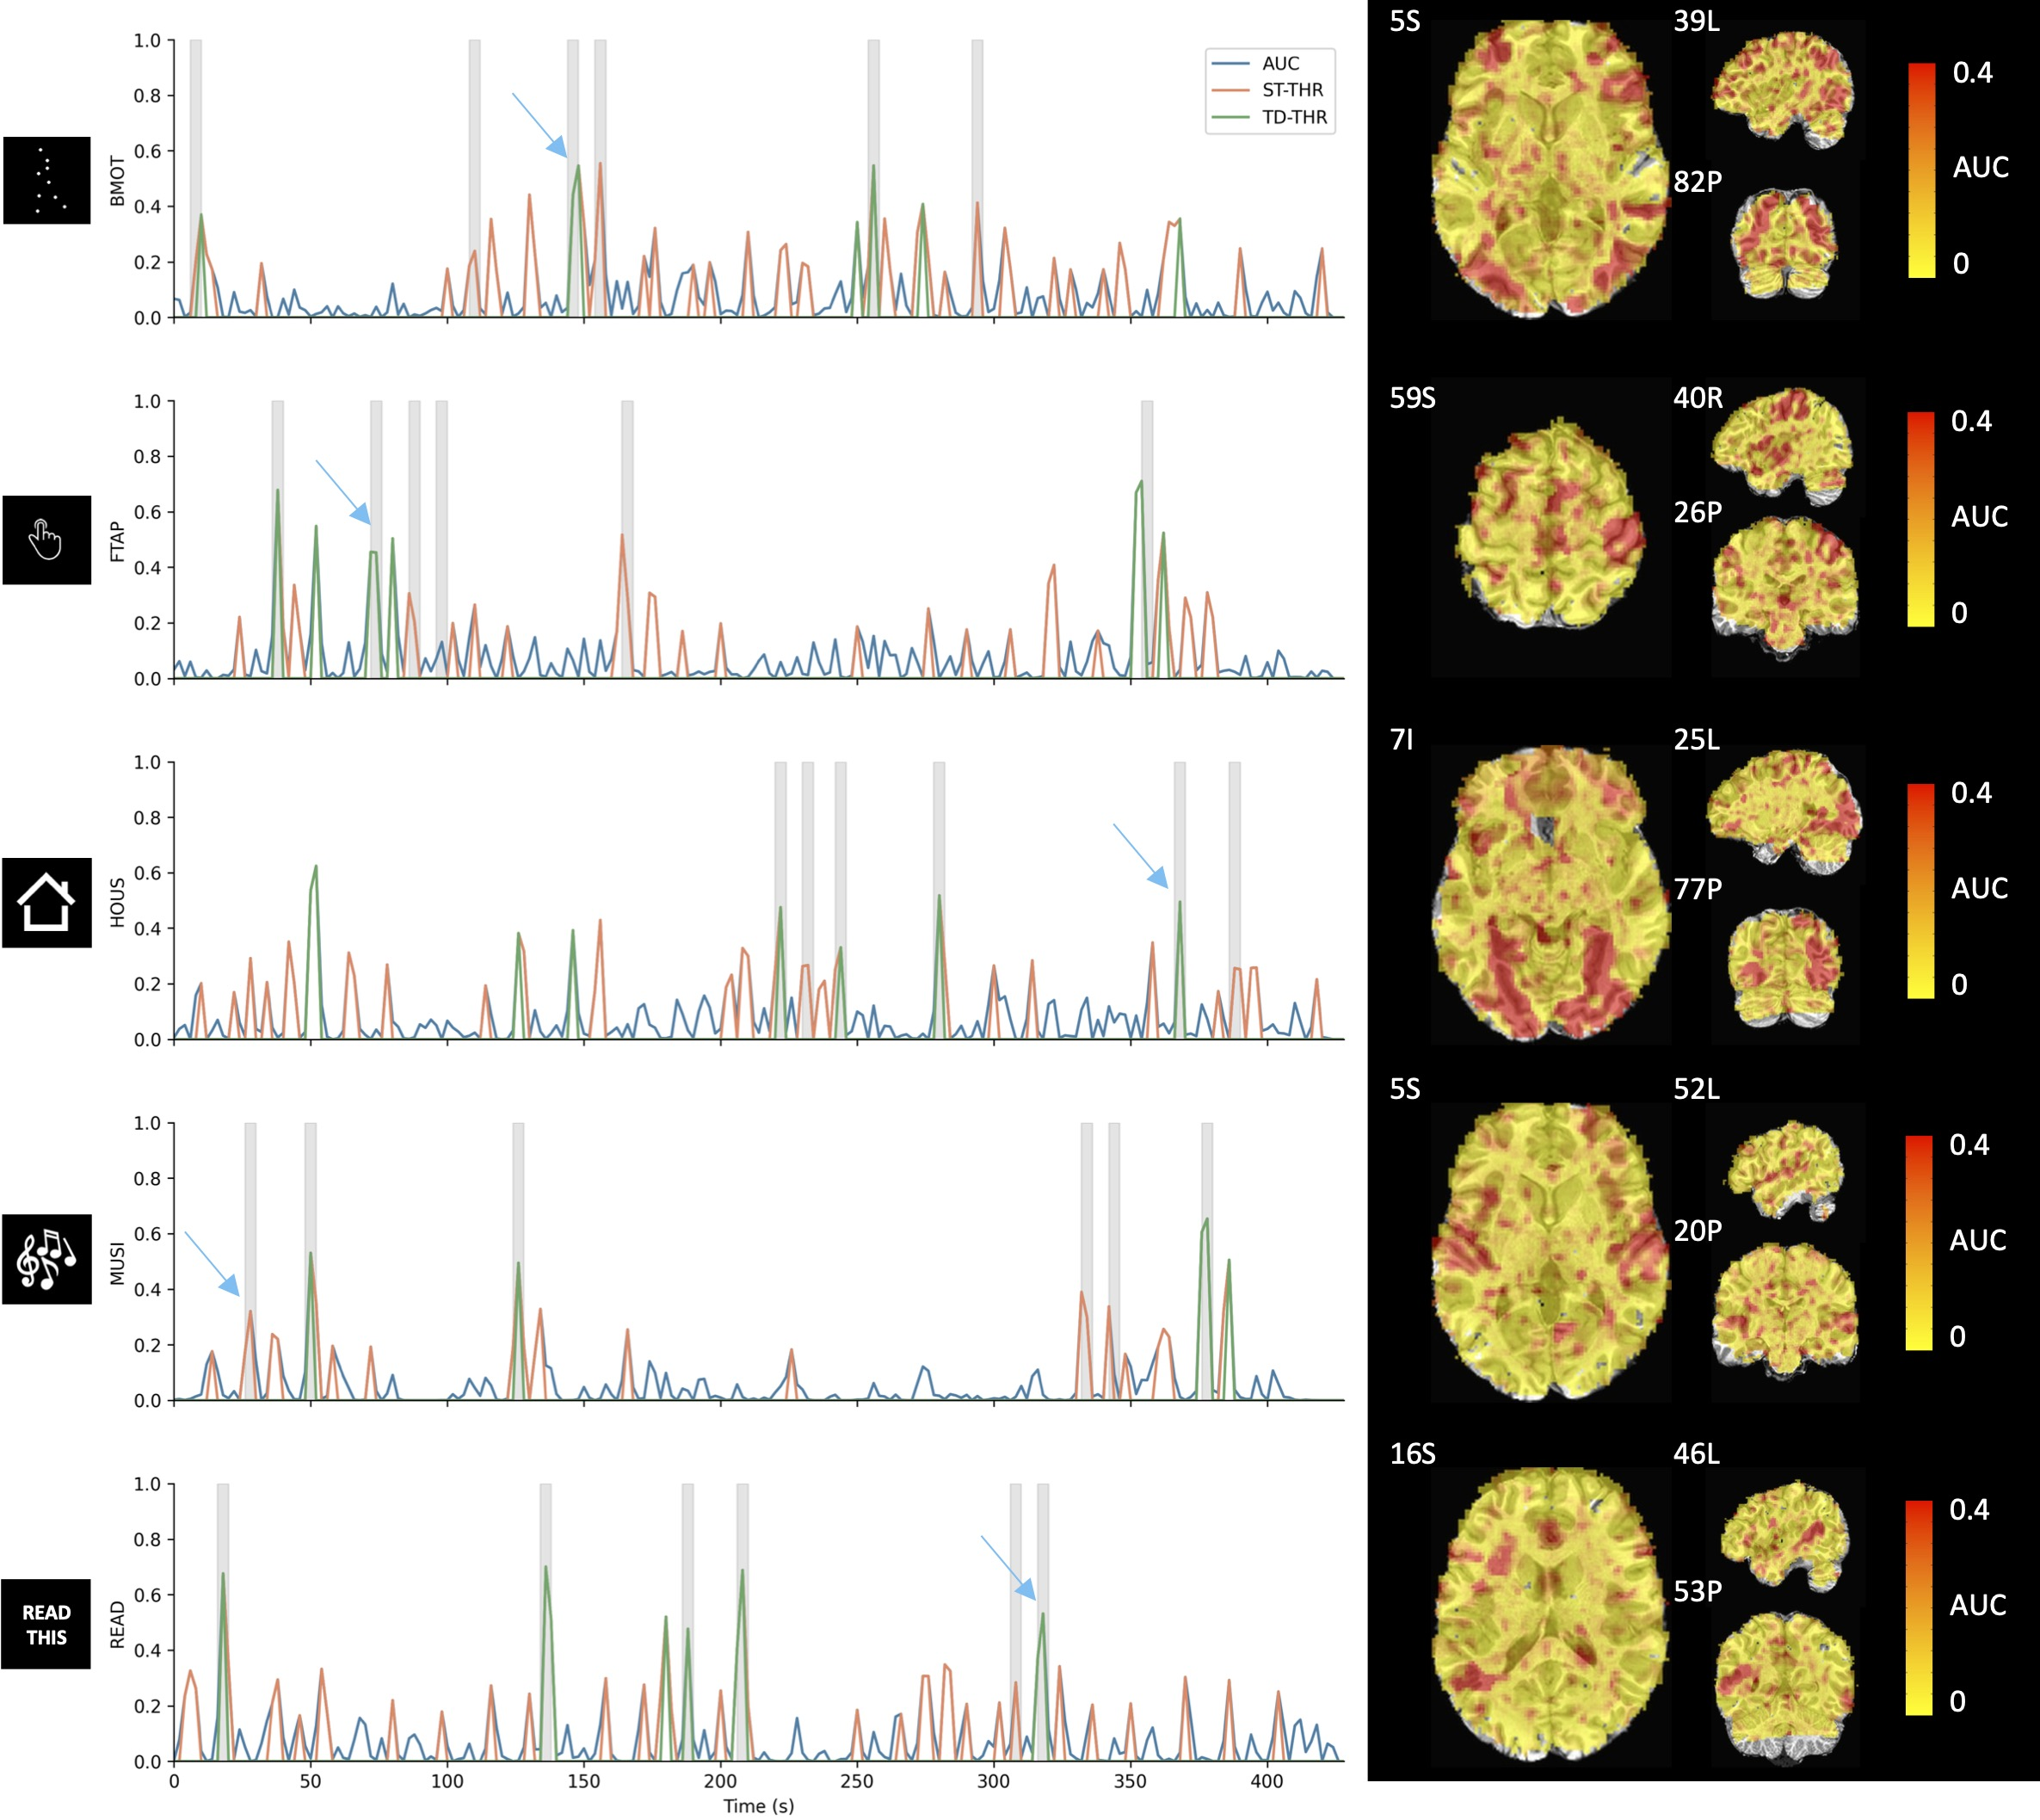
\includegraphics[width=\textwidth]{figures/multivariate/auc.jpg}}
    \caption{\textbf{Left:} Original (blue), ST thresholded (orange) and TD
    thresholded (green) AUC time-series for a representative voxel for each task
    in the paradigm ($\rho=0.5$). Note that the three time-series are overlaid;
    i.e., the static and time-dependent time-courses are thresholded versions of
    the original AUC. Gray blocks depict the onset and duration of each trial.
    \textbf{Right:} AUC maps at the time-points signaled by the blue arrows.}
\label{fig:auc}
\end{figure}

\cref{fig:rho_comparison} displays the comparison of the $\Delta R_2^*$
maps obtained by solving the inverse problem in
Eq.~\eqref{eq:multivariate_multi-echo_inverse_problem} with a fixed selection of
$\lambda$ (1$^{st}$ row) and with the use of stability selection (2$^{nd}$,
3$^{rd}$ and 4$^{th}$ rows) for $\rho = \{0, 0.5, 1\}$. The $\Delta R_2^*$ maps
obtained with a fixed selection of $\lambda$ equal to the noise estimate of the
first echo volume (1$^{st}$ row) are very sensitive to the selection of $\rho$.
Similar observations were obtained with other values of $\lambda$. With a
selection of $\rho = 1$, only the $\ell_1$-norm regularization term is applied,
which produces $\Delta R_2^*$ maps with few non-zero coefficients. With $\rho =
0$, only the $\ell_{2,1}$-norm spatial regularization is applied, which yields a
$\Delta R_2^*$ map that covers the entire brain and does not exhibit a spatial
pattern in concordance with the task. However, a selection of $\rho = 0.5$
yields a $\Delta R_2^*$ map that is more similar to the activity maps often
observed when participants are asked to look at the image of a house, depicting
negative $\Delta R_2^*$ in bilateral fusiform regions. In contrast, the use of
stability selection yields AUC maps (row 2) and the corresponding $\Delta R_2^*$
maps after each thresholding strategy (rows 3-4) reveal activation patterns
concordant with those often seen for viewing houses regardless of the selection
of $\rho$. In other words, the $\Delta R_2^*$ maps obtained with stability
selection are less sensitive to the selection of $\rho$ while obviating the need
to choose $\lambda$. In fact, the spatial correlations between the AUC maps for
each pair of $\rho$'s were nearly equal to 1 for all time points (average
correlations are 0.97 between $\rho=\{0,0.5\}$, 0.98 between $\rho=\{0,1\}$, and
0.97 between $\rho=\{0.5,1\}$). In addition, it can be seen that using a TD
threshold yields BOLD signal changes that are more confined to the expected
areas in bilateral fusiform cortices than the ST threshold. Due to the high
similarity of the AUC maps for any value of $\rho$, only the results for
$\rho=0.5$ are discussed hereinafter.

\begin{figure}[ht!]
    \centerline{\includegraphics[width=\textwidth]{figures/multivariate/rho_comparison.jpg}}
    \caption{Comparison of the $\Delta R_2^*$ maps obtained with a fixed
    selection of $\lambda$ (row 1) and the use of stability selection (rows 2-4:
    AUC, stability selection with static thresholding (ST), and stability
    selection with time-dependent thresholding (TD)) for $\rho = 0$ (column 1),
    $\rho = 0.5$ (column 2), and $\rho = 1$ (column 3). These maps correspond to
    a single-trial event of the house-viewing task (HOUS).}
\label{fig:rho_comparison}
\end{figure}

\cref{fig:artifacts} provides an in-depth view of how the time-dependent
thresholding operates when motion- and respiration-related artifacts are present
in the data. The grayplot \citep{Power2017simpleusefulway} in
\cref{fig:artifacts}A clearly shows bands spanning throughout the entire brain
that illustrate significant changes in the amplitude of the signal. The source
of these signal changes can be attributed to head motion events (see Euclidean
norm in \cref{fig:artifacts}C) and deep breaths (see arrows for respiration
volume signal \citep{Chang2009Influenceheartrate} in \cref{fig:artifacts}D). The
respiration-related events cause a drop in the global signal (see
\cref{fig:artifacts}B) seconds after the peak in the respiration volume signal.
Interestingly, our results show a decrease in the equivalent ST percentile that
corresponds to the 95th TD threshold (\cref{fig:artifacts}E) at the instances of
these large respiratory-related events. This decrease can also be observed in
the corresponding AUC value of the TD thresholding strategy as shown in
\cref{fig:artifacts}F. The distributions of AUC values at the time-points with
respiratory- and motion-related artifacts have a shorter tail than the
distribution of the AUC values at the time-points where subjects performed the
task. Hence, in these events the TD thresholding strategy is able to adjust the
threshold so that the final estimates of $\Delta R_2^*$ specifically capture
task-activated voxels while excluding voxels that are affected by artifacts. The
higher specificity of the TD thresholding strategy can be clearly seen in the
\acrshort*{roc} values shown in \cref{fig:artifacts}H-L. The use of stability
selection with the TD threshold yields more specific estimates of $\Delta R_2^*$
than with ST thresholding or the original ME-SPFM method, while the sensitivity
is slightly reduced. On the other hand, the use of stability selection with a ST
threshold improves the sensitivity of the $\Delta R_2^*$ estimates compared to
the original ME-SPFM technique while preserving its specificity.

\begin{figure}[ht!]
    \centerline{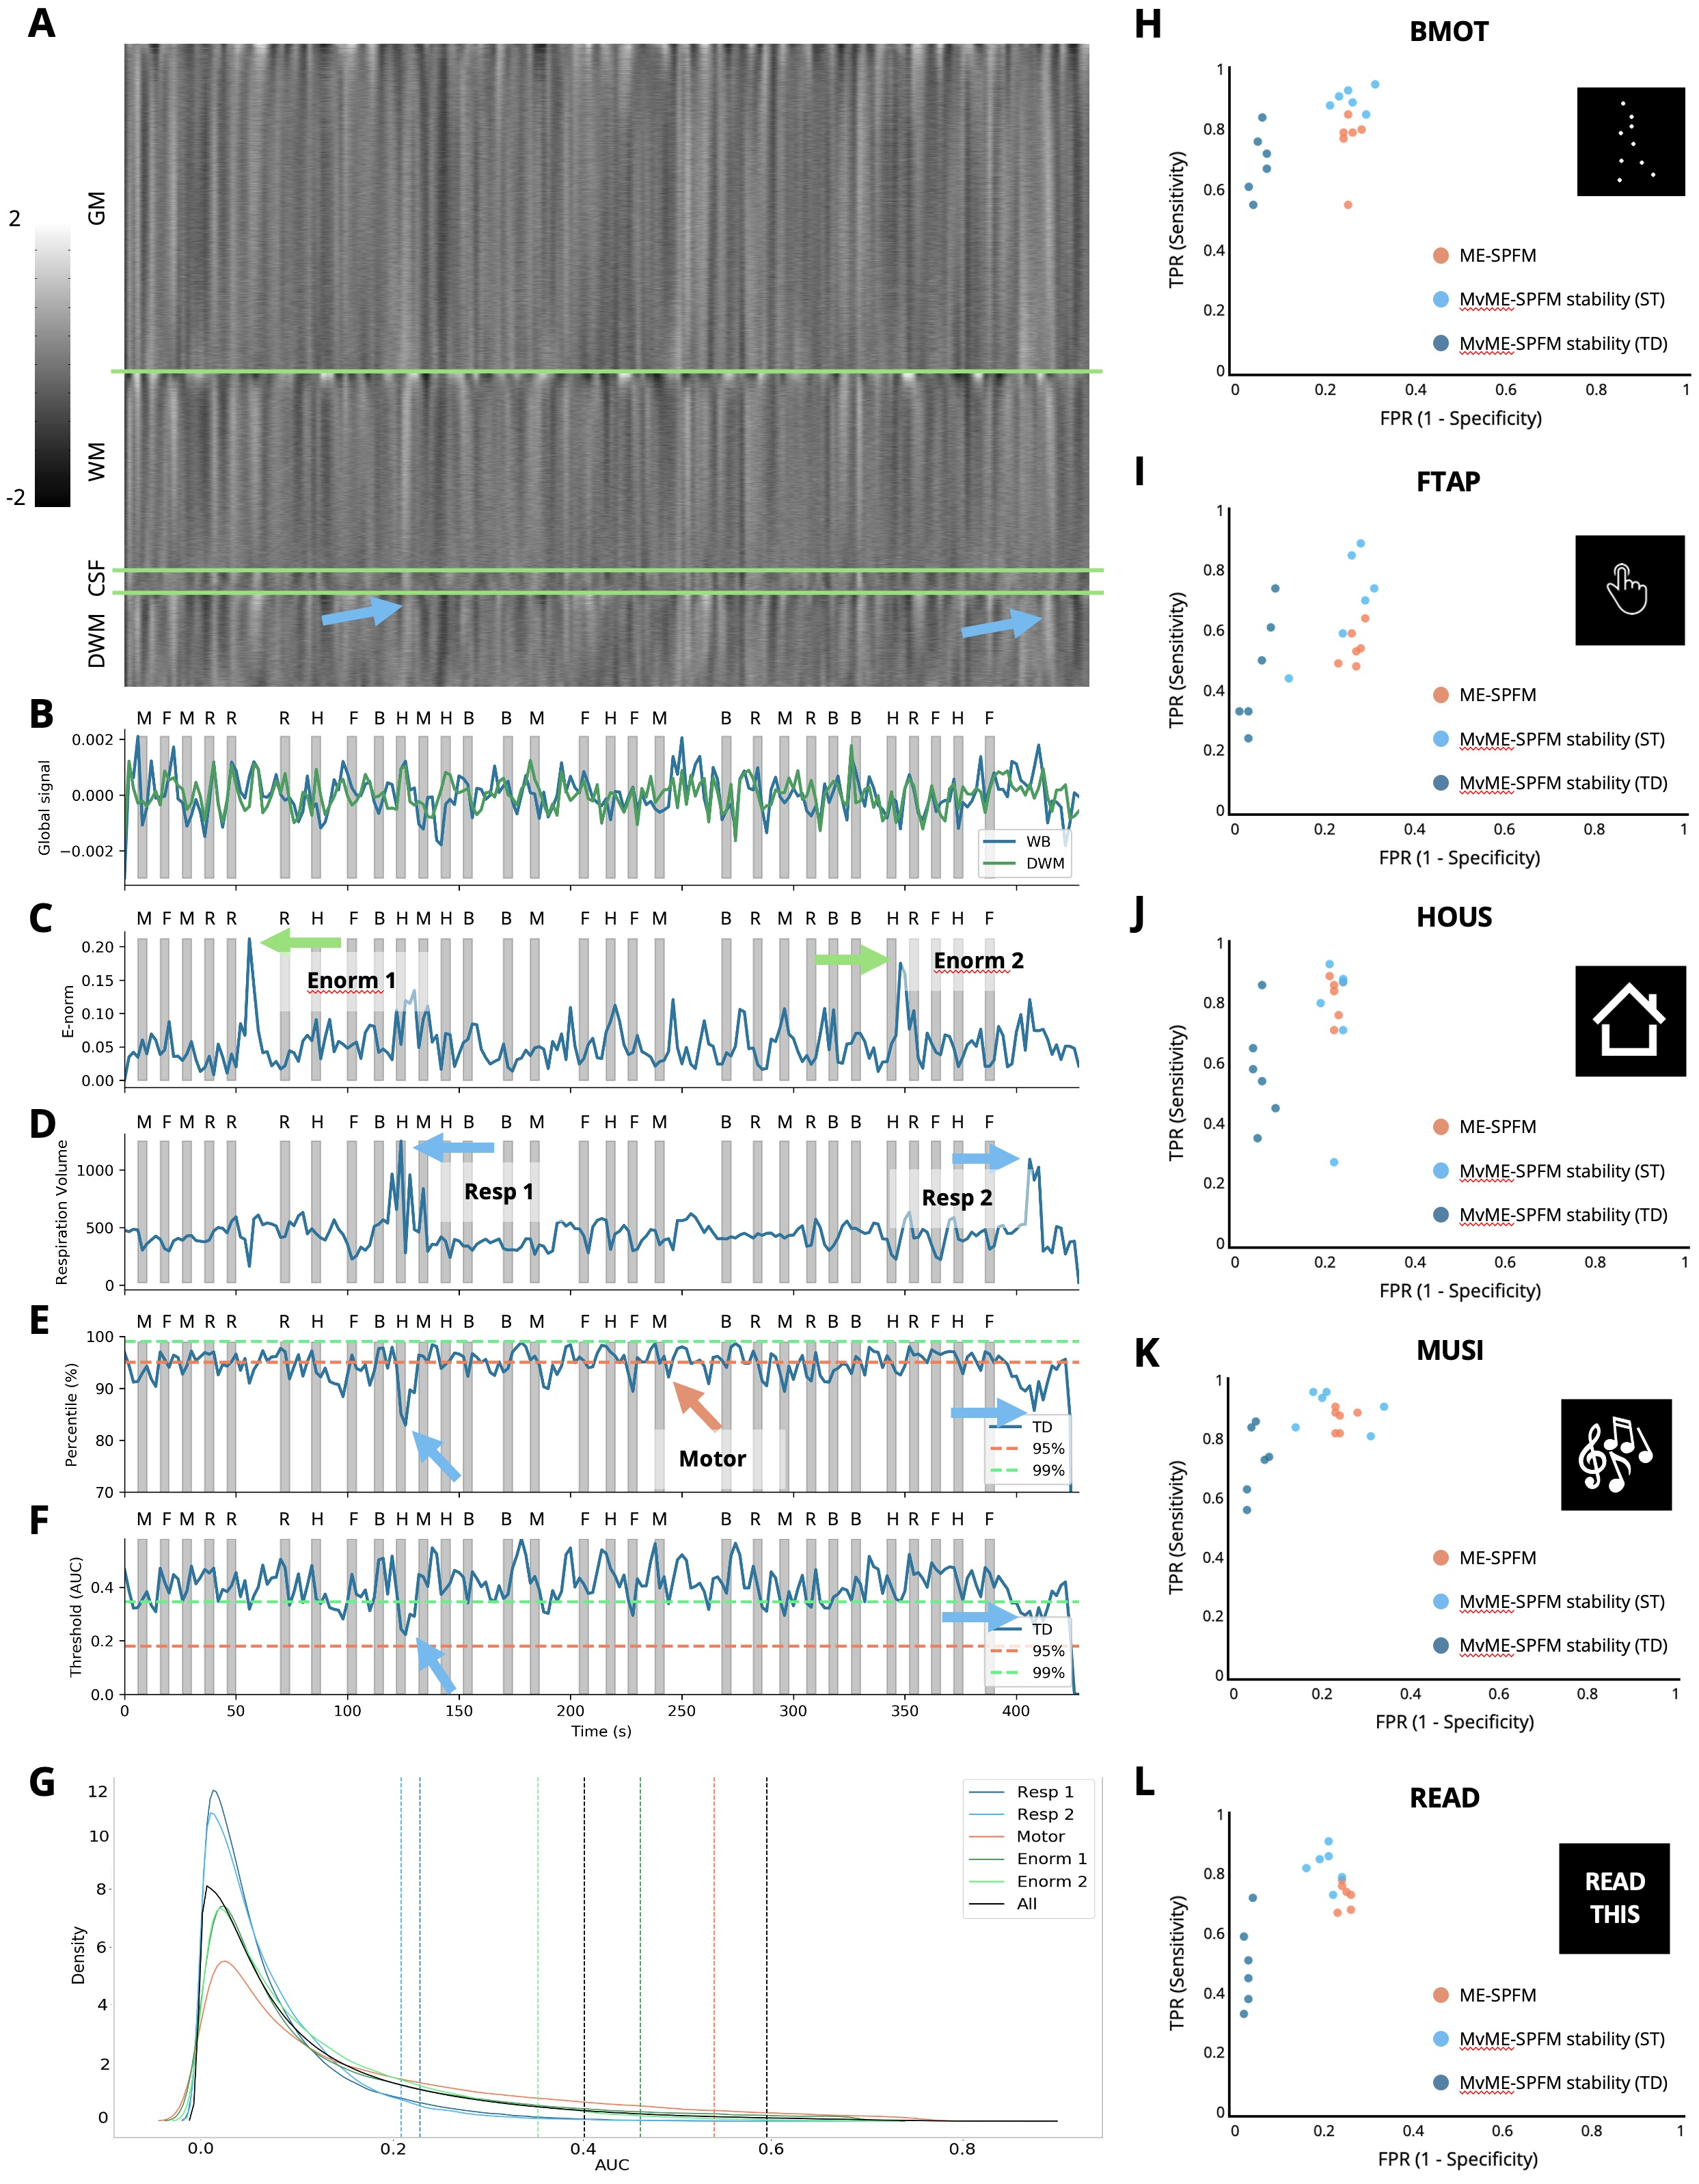
\includegraphics[width=\textwidth]{figures/multivariate/artifacts.jpg}}
    \caption{Representative subject with motion and respiration artifacts.
    \textbf{A:} Grayplot of the second echo volume. The grayplot is divided into
    4 sections: gray matter (GM), white matter (WM), cerebrospinal fluid (CSF),
    and deep white matter (DWM). \textbf{B:} Time-series of the global signal
    calculated in the whole brain (WB, blue) and the deep white matter (DWM,
    green).}
\label{fig:artifacts}
\end{figure}
\begin{figure}[ht!]
    \contcaption{ \textbf{C:} Euclidean norm (e-norm) of the temporal derivative
    of the realignment parameters. \textbf{D:} respiration volume signal.
    \textbf{E:} AUC percentile corresponding to the time-dependent threshold
    (lines at 95th and 99th percentiles are shown for reference).\textbf{F:} AUC
    values corresponding to the time-dependent threshold are shown in blue. The
    horizontal dashed lines indicate the 95th (orange) and 99th (green)
    percentiles corresponding to ST thresholding. Gray bars in \textbf{B-F}
    indicate the onset and duration of each trial in the paradigm, with their
    respective initials on top. Blue arrows point out two respiration-related
    events, green arrows point out two motion-related events, and the orange
    arrow points out a finger-tapping event. \textbf{G:} Probability density
    functions (estimated by kernel density estimate) of the AUC values
    corresponding to the instances of the two respiratory-related events (blue
    lines), a representative time-point of one finger-tapping trial (orange
    line), the two largest peaks in the e-norm trace (green lines), and the
    overall AUC distribution (black). The corresponding coloured vertical dashed
    lines indicate the AUC value for the 95th percentile of the TD thresholding
    approach, along with the 95th and 99th AUC values of ST thresholding.
    \textbf{H-L:} Receiver operating characteristic (ROC) values for the
    original ME-SPFM (orange), and proposed MvME-SPFM technique with the use of
    stability selection with the ST (light blue) and TD (dark blue) thresholding
    approaches for this dataset. The ROC plots depict the sensitivity and
    specificity of the methods at correctly estimating the activity maps that
    correspond to the 6 trials of each task in the paradigm.}% Continued caption
\end{figure}

\cref{fig:dr2_time_series} depicts the time-series of the estimated
$\Delta R_2^*$ and denoised BOLD, i.e., $\Delta R_2^*$ convolved with the HRF,
for a representative voxel of each task for the subject depicted in
\cref{fig:artifacts} and \cref{fig:activity_maps} and compared to a
reference voxel in the lateral ventricles. The location of the voxels is shown
in the corresponding maps in \cref{fig:activity_maps}. The ST thresholding
approach detects $\Delta R_2^*$ events of the activity-inducing signal that
correctly match the timings of the stimuli (i.e., high temporal sensitivity),
but also shows events that occur in the resting state and do not coincide with
any activity-evoking trial. Based on comparison with the events detected in the
time series extracted from the lateral ventricles, it can be conjectured that
some of these events might be due to artifactual and physiological fluctuations
that remain in the signal after preprocessing. On the other hand, $\Delta R_2^*$
values estimated with the TD thresholding approach match the timings of the
stimuli almost perfectly with few missed trials (high temporal specificity).
This is supported by the few $\Delta R_2^*$ events obtained for the reference
voxel in the ventricles. Likewise, the denoised BOLD time-series obtained with
the TD thresholding approach clearly describes signal changes associated with
the trials, whereas the denoised BOLD time-series estimated with the ST
thresholding strategy fits the original data very closely, which could be
interpreted as a signature of overfitting.

\begin{figure}[ht!]
    \centerline{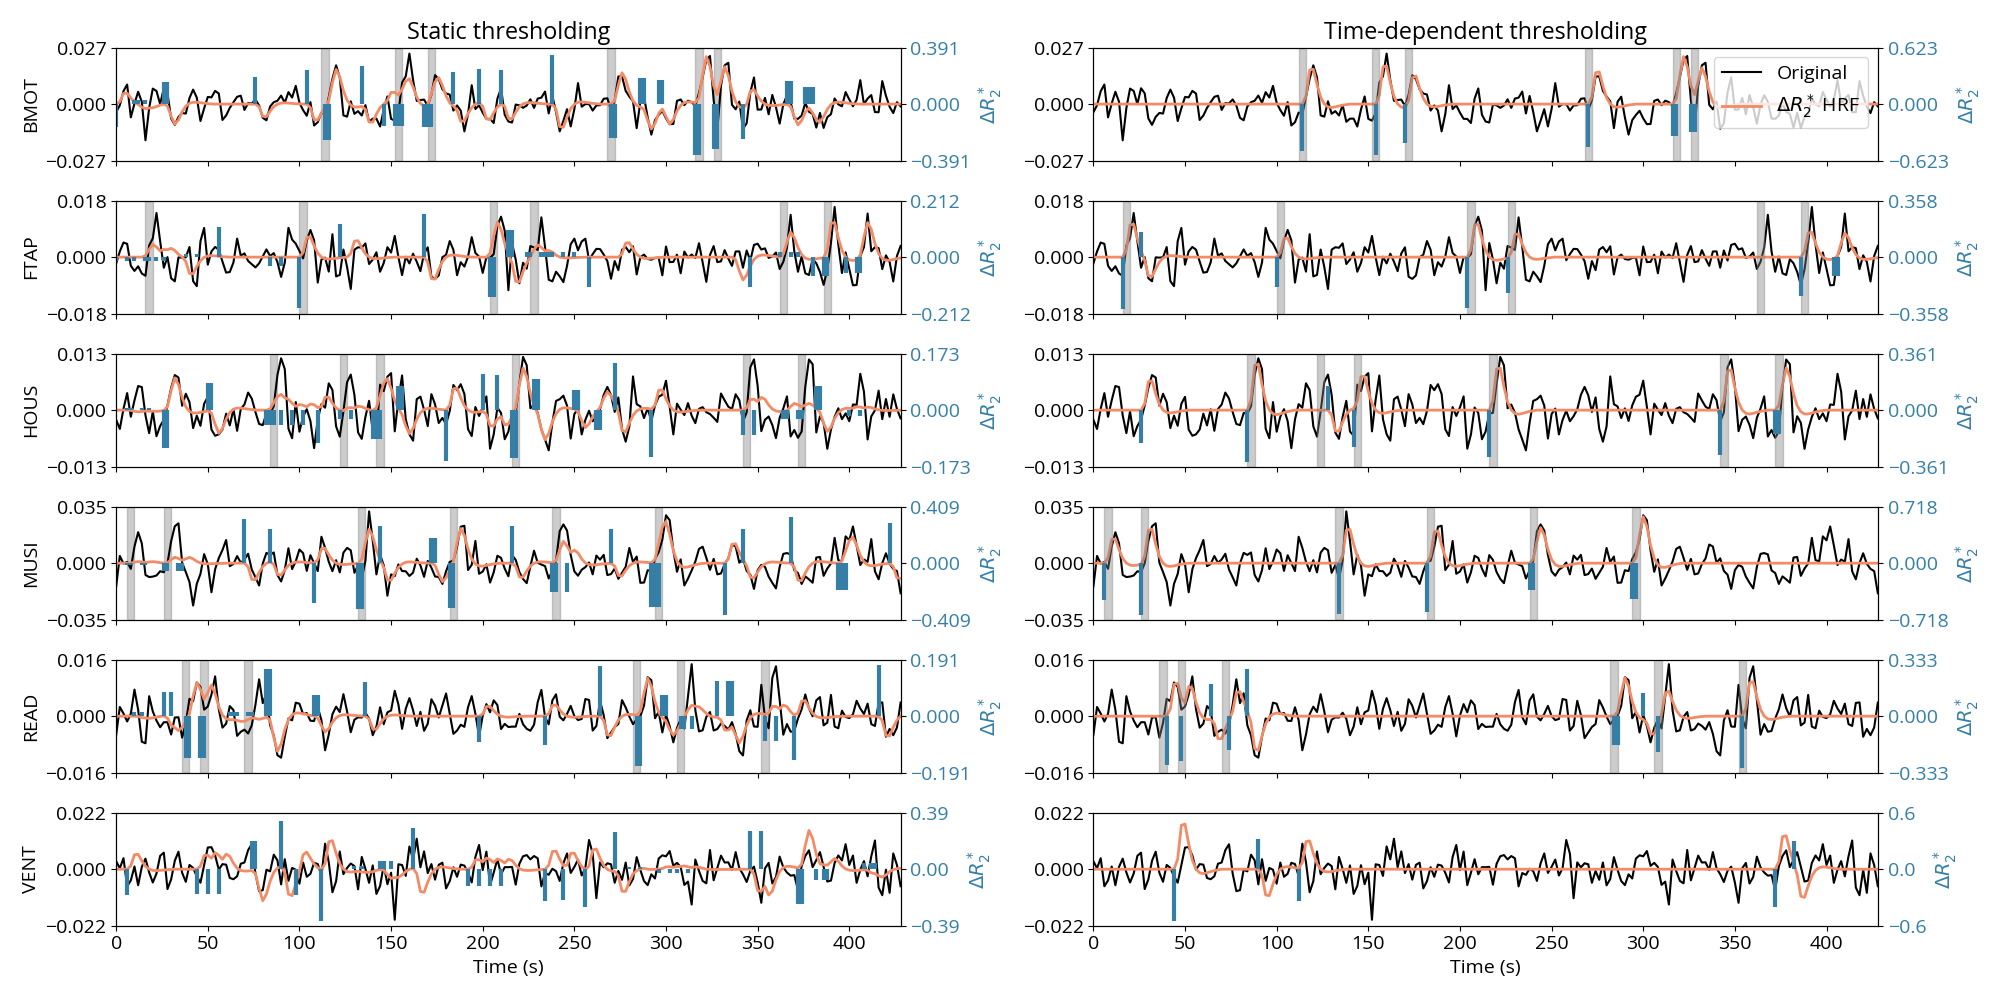
\includegraphics[width=\textwidth]{figures/multivariate/dr2_time_series.png}}
    \caption{Comparison of the estimated $\Delta R_2^*$ (blue) and denoised BOLD
    (orange), i.e., $\Delta R_2^*$ convolved with the HRF, time-series when
    employing the ST (left) and TD (right) thresholding approches, for
    representative voxels of each task (rows) as well as one voxel from the
    lateral ventricle for reference. The estimates shown here were obtained with
    $\rho=0.5$. The preprocessed time series is shown in black. The gray bars
    indicate the onset and duration of each trial for each task of the
    experimental paradigm.}
\label{fig:dr2_time_series}
\end{figure}

\cref{fig:activity_maps} illustrates the activation maps of representative
single-trial events of each task for the same subject depicted in
\cref{fig:artifacts}. The activation maps of the proposed MvME-SPFM formulation
were compared using the two thresholding approaches with the activation maps
obtained with a single-trial GLM and the previous ME-SPFM approach. While all
PFM methods exhibit activation maps that highly resemble those obtained with the
single-trial GLM analysis, differences between the methods can be observed. For
instance, although the use of stability selection with a ST thresholding
approach yields maps with clusters of activation of comparable size and location
to those found with ME-SPFM, in certain noisy trials (e.g., see HOUS-Trial 1),
the ST-thresholding MvME-SPFM maps can yield reduced spatial specificity,
probably related to spurious, scattered changes in $R_2^*$. Across all tasks,
the maps obtained with TD thresholding exhibit a notably larger resemblance to
the single-trial GLM, showing higher spatial specificity and lower sensitivity
compared to the other two PFM methods. 

To further evaluate the proposed MvME-SPFM, the motor task of a single subject
(\textit{100206}) extracted from the Human Connectome Project (HCP) dataset
\citep{VanEssen2013WUMinnHuman} was analyzed. The data was 3 min 24 s long
(after removing the first 10 seconds for steady magnetization) with a TR of 0.72
s, a multi-band factor of 8 and a spatial resolution of $2\times2\times2$
mm$^3$. The images were already preprocessed using a standard HCP pipeline
including realignment, coregistration, spatial normalization and smoothing. The
task was composed of 5 blocks of 12 s each, preceded by a 3 s cue indicating the
task to be performed by the participant. The conditions in each 5-second block
were: left hand finger tapping, right hand finger tapping, left foot movement,
right foot movement, and tongue movement. The process was repeated once more,
resulting in a total of 10 blocks. We adjusted the signal model in
Eq.~\eqref{eq:multivariate_multi-echo_model} to be used with single-echo data as
described in
\citep{Gaudes2013Paradigmfreemapping,Urunuela2023HemodynamicDeconvolutionDemystified}

The accurate performance of the proposed MvME-SPFM method observed in the
multi-echo fMRI data is consistent with the results found in the single-echo
data from the Human Connectome Project. \cref{fig:hcp_motor} depicts the
single-trial activity maps obtained with a GLM and the proposed approach with
stability selection and both ST and TD thresholding. In general, the activity
maps obtained with the proposed method are highly comparable to the single-trial
GLM activation maps. Importantly, the proposed method showed a larger
sensitivity to detect the activity evoked by the motor task for certain trials
than the timing-aware GLM analysis. For instance, the Mv-SPFM activation maps of
the second trial for the left hand finger tapping condition shows more BOLD
activity in motor regions of the right precental gyrus, which is barely seen in
the corresponding single-trial GLM map.

\begin{figure}[t!]
    \centerline{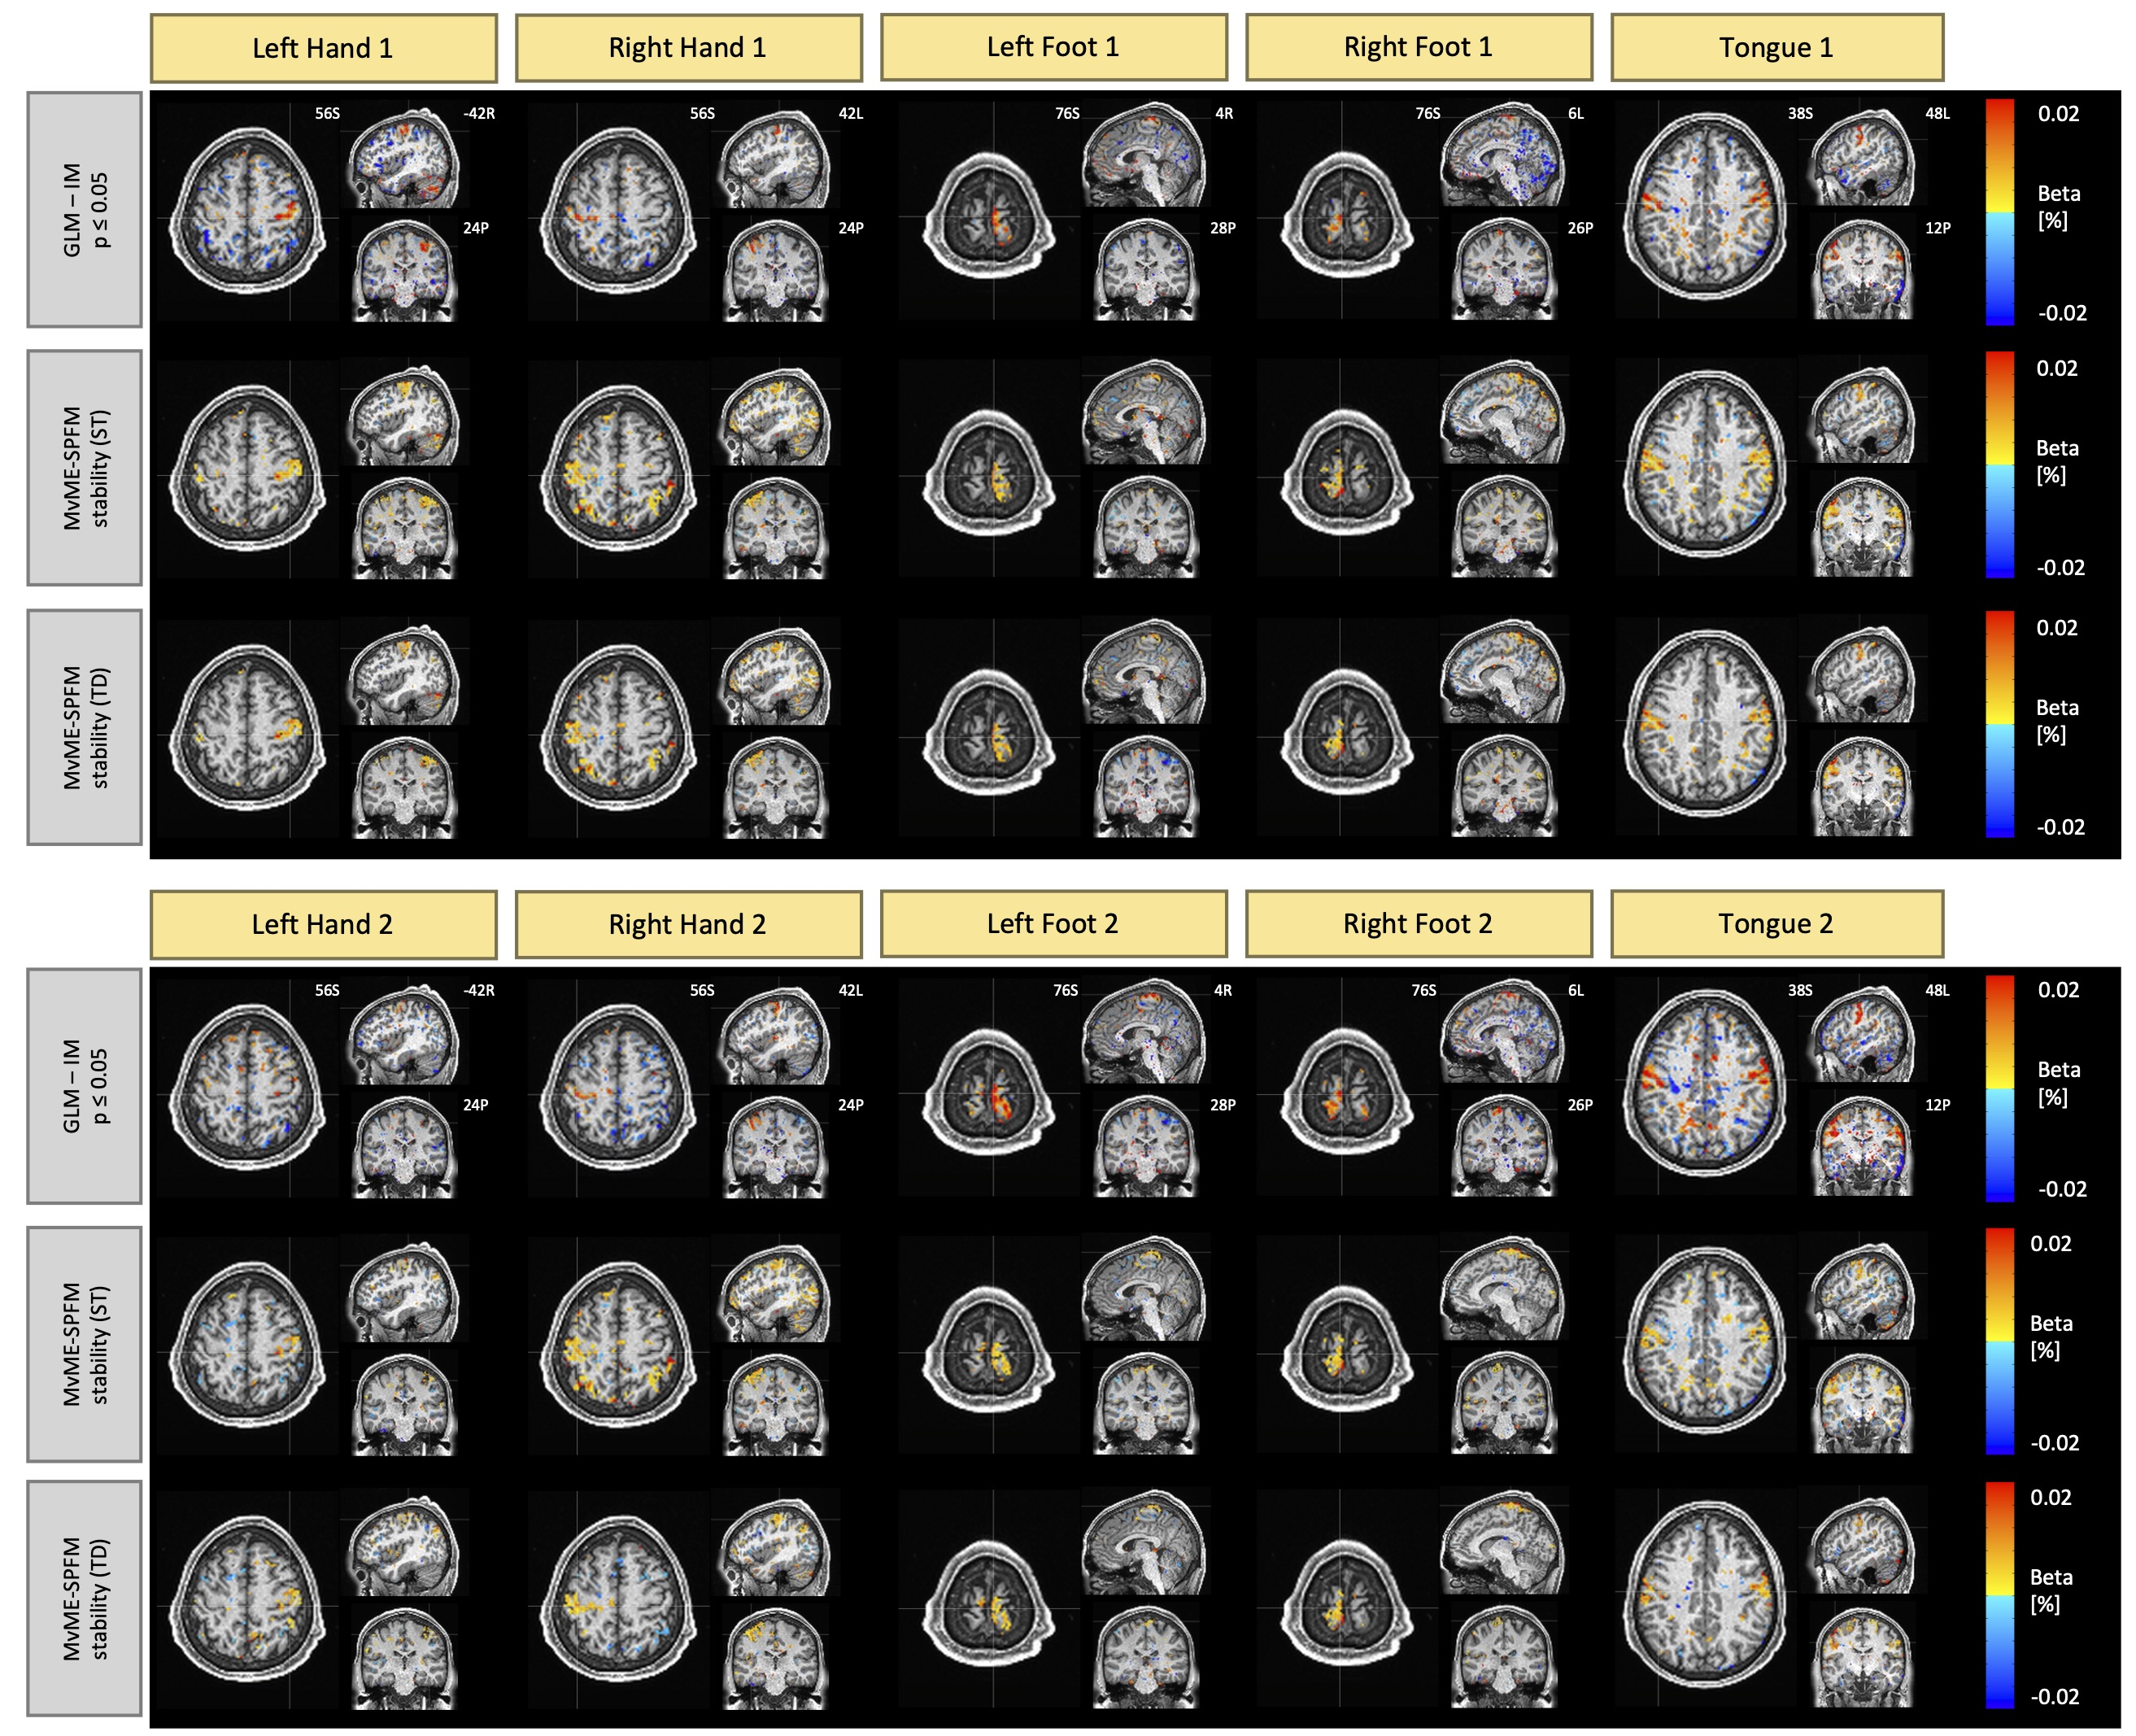
\includegraphics[width=\textwidth]{figures/multivariate/hcp_motor.jpg}}
    \caption{Single-trial activity maps estimated for the single-echo motor task
    data from the Human Connectome Project.Row 1 depicts the activation maps
    obtained with a single-trial GLM ($p \leq 0.05$), row 2 depicts the maps
    detected with the novel Mv-SPFM technique with stability selection,
    $\rho=0.5$ and a static threshold (ST), and row 3 illustrates the results
    using a time-dependent threshold (TD). The activity maps corresponding to
    the first trial are shown on top, and the activity maps corresponding to the
    second trial are shown on the bottom.}
\label{fig:hcp_motor}
\end{figure}

\begin{figure}[ht!]
    \centerline{\includegraphics[width=\textwidth]{figures/multivariate/activity_maps.jpg}}
    \caption{Comparison of single-trial activation maps obtained with a GLM (row
    1) thresholded at $p \leq 0.05$, the original ME-SPFM formulation with a
    fixed selection of $\lambda$ (row 2), the novel MvME-SPFM technique with
    stability selection, $\rho=0.5$ and a static threshold (ST, row 3), and
    using a time-dependent threshold (TD, row 4). A representative trial is
    shown for each task. All the maps correspond to the same subject and run
    shown in \cref{fig:artifacts}.}
\label{fig:activity_maps}
\end{figure}

As illustrated in \cref{fig:dice}, the Dice coefficient between the
estimated single-trial $\Delta R_2^*$ activity maps and the reference GLM
activity maps ($p \leq 0.05$) demonstrates only a slight improvement over the
original ME-SPFM formulation when employing an ST thresholding approach with the
novel MvME-SPFM technique. In contrast, the Dice coefficients obtained with TD
thresholding show a very notable increase of nearly 50\% in the median of the
distribution of Dice coefficients compared with the original ME-SPFM approach.
Similarly, the sensitivity and specificity distributions of ST thresholding
demonstrate a slight improvement with respect to the original ME-SPFM
formulation. On the other hand, the use of TD thresholding offers nearly perfect
specificity ($\geq 95\%$) at the cost of reduced sensitivity across all
experimental conditions. Hence, increasing the specificity of the $\Delta R_2^*$
maps is more beneficial for increasing the concordance with the GLM maps than
increasing the sensitivity. 

The receiver operating characteristic (ROC) values in \cref{fig:roc} corroborate
the previous observations regardless of the value of $\rho$ used in the
MvME-SPFM method. The estimates obtained with the ST threshold reveal an overall
higher sensitivity and a slightly higher specificity compared to the original
ME-SPFM technique. In contrast, the ROC values for the TD thresholding approach
show a clear improvement in specificity but lower sensitivity. These findings
are in line with the results shown in \cref{fig:rho_comparison},
\cref{fig:activity_maps} and \cref{fig:dr2_time_series}, as the Dice and ROC
values certify that the use of stability selection yields robust activation maps
regardless of the selection of the spatial regularization term $\rho$ and
obviating the need to choose the temporal regularization parameter $\lambda$. An
interactive version of \cref{fig:dice} and \cref{fig:roc} is available in the
following GitHub repository: \url{https://github.com/eurunuela/MvMEPFM_figures}.

\begin{figure}[ht!]
    \centerline{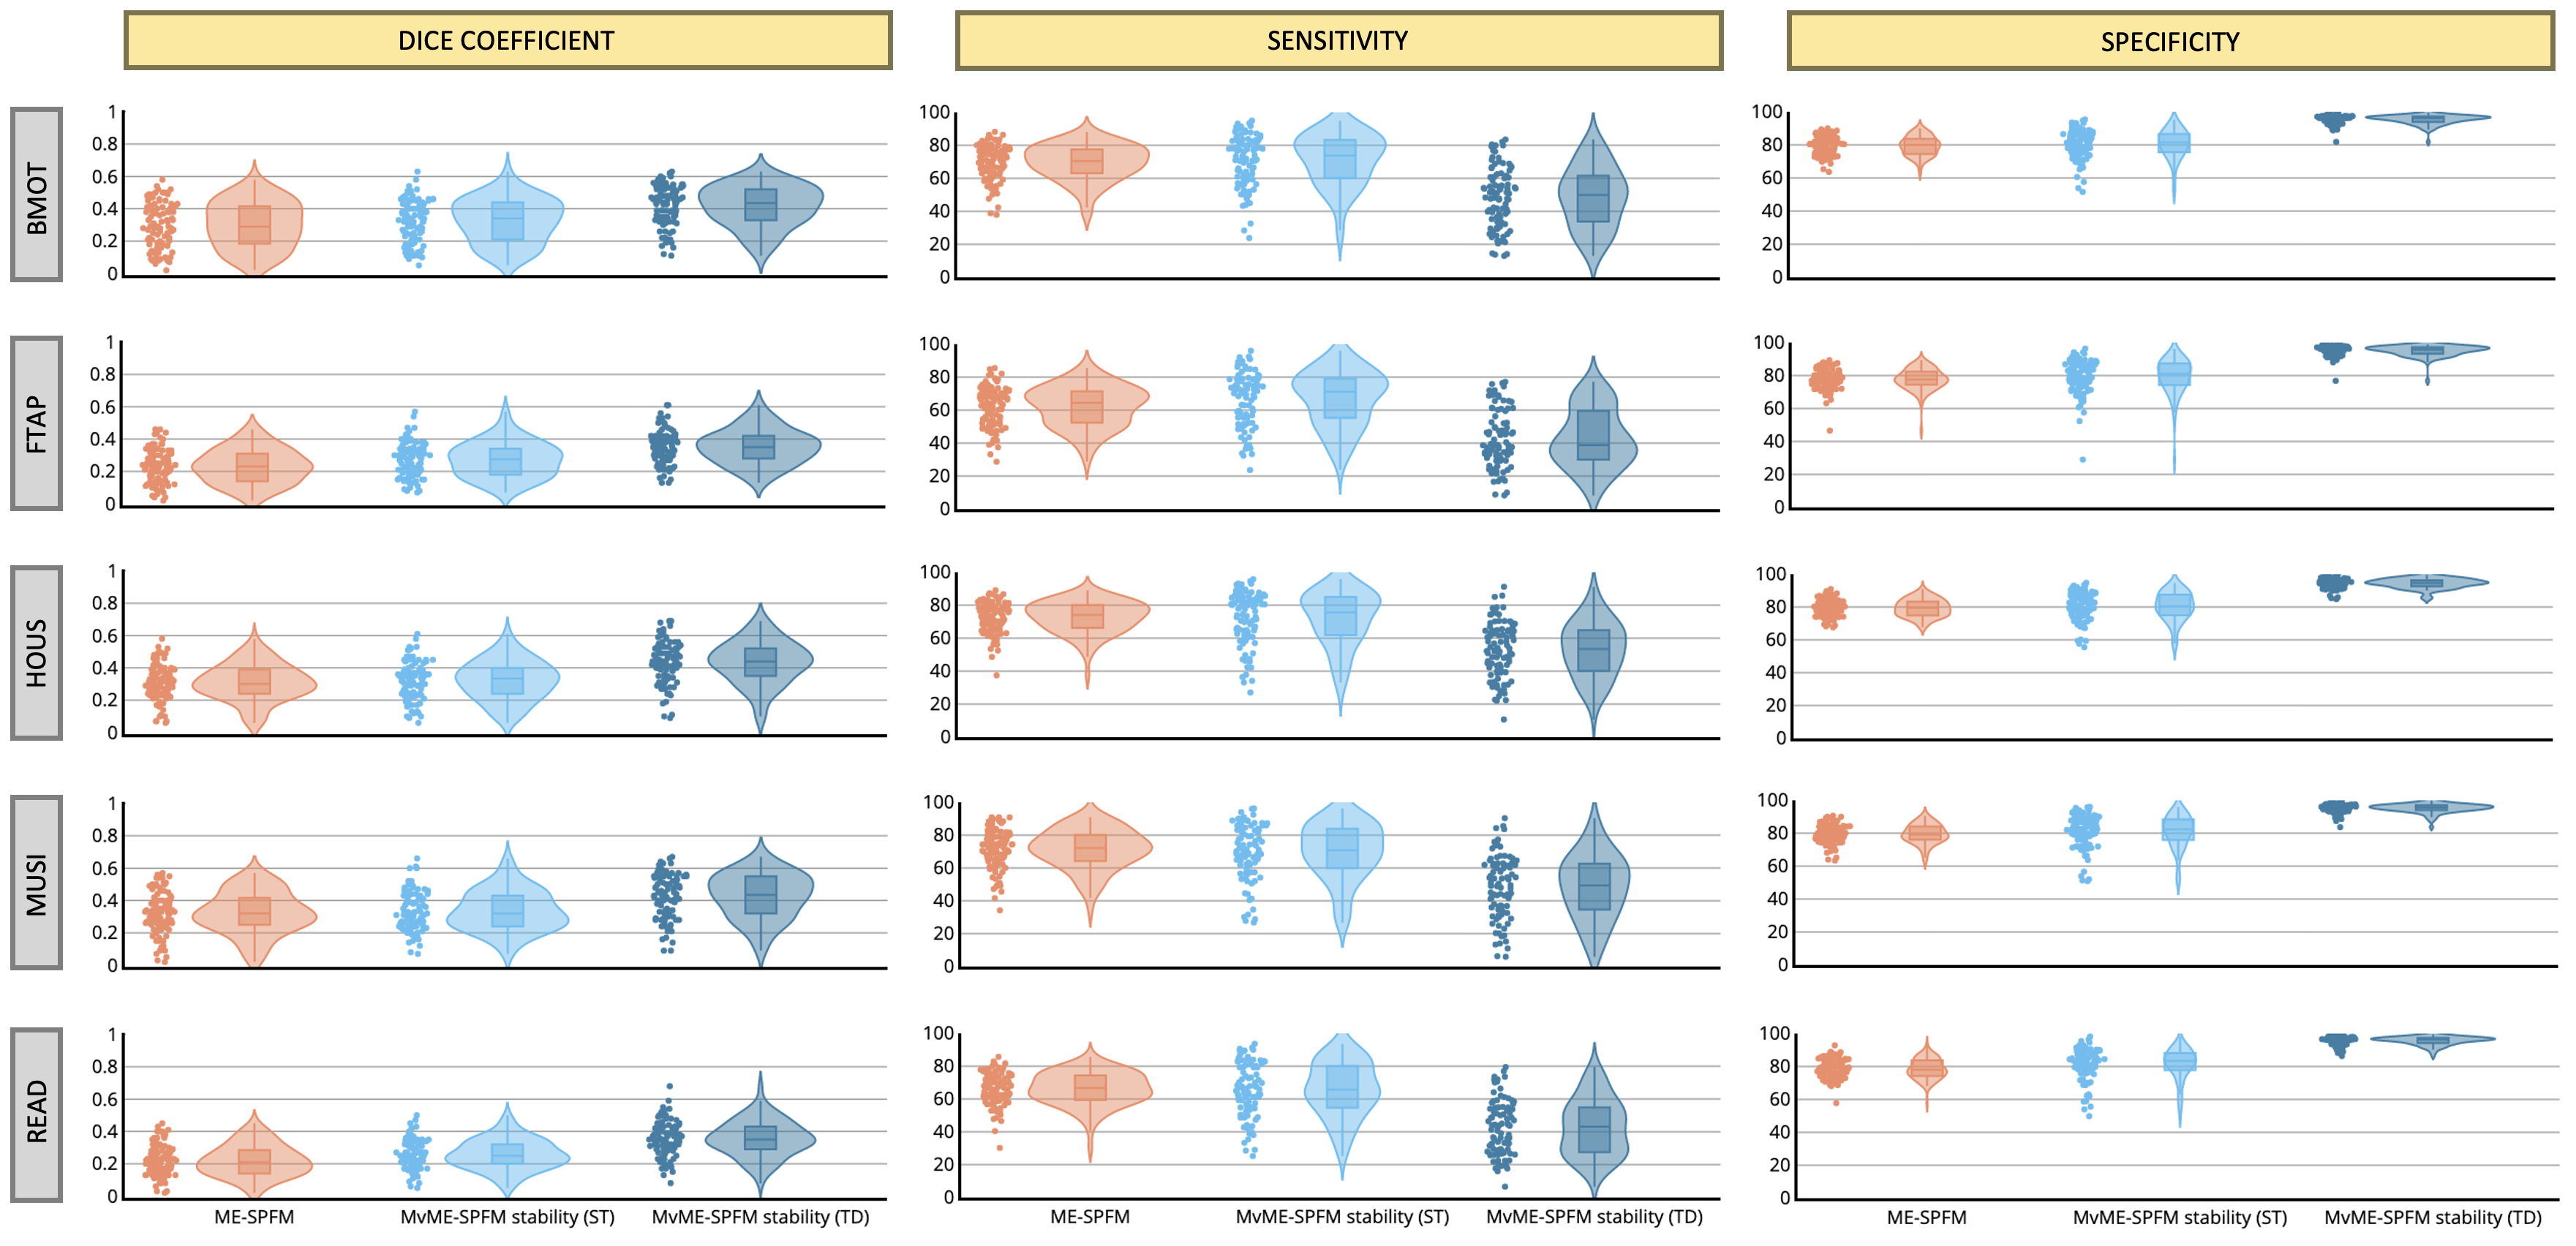
\includegraphics[width=\textwidth]{figures/multivariate/dice.png}}
    \caption{Dice coefficient (i.e., spatial overlap), sensitivity and
    specificity coefficients of the single-trial activation maps for each of the
    experimental conditions obtained with ME-SPFM, MvME-SPFM with stability
    selection and a static thresholding approach (ST), and MvME-SPFM with
    stability selection and a time-dependent thresholding approach (TD). These
    metrics were obtained with a selection of $\rho = 0.5$. Reference activation
    maps were obtained with a single trial GLM analysis and thresholded at
    uncorrected $p \leq 0.05$. The density plot shows the shape of the
    distribution of the Dice coefficients, and the box plot depicts the median
    with a solid line, with each box spanning from quartile 1 to quartile 3. The
    whiskers extend to 1.5 times the interquartile range.}
\label{fig:dice}
\end{figure}

\begin{figure}[ht!]
    \centerline{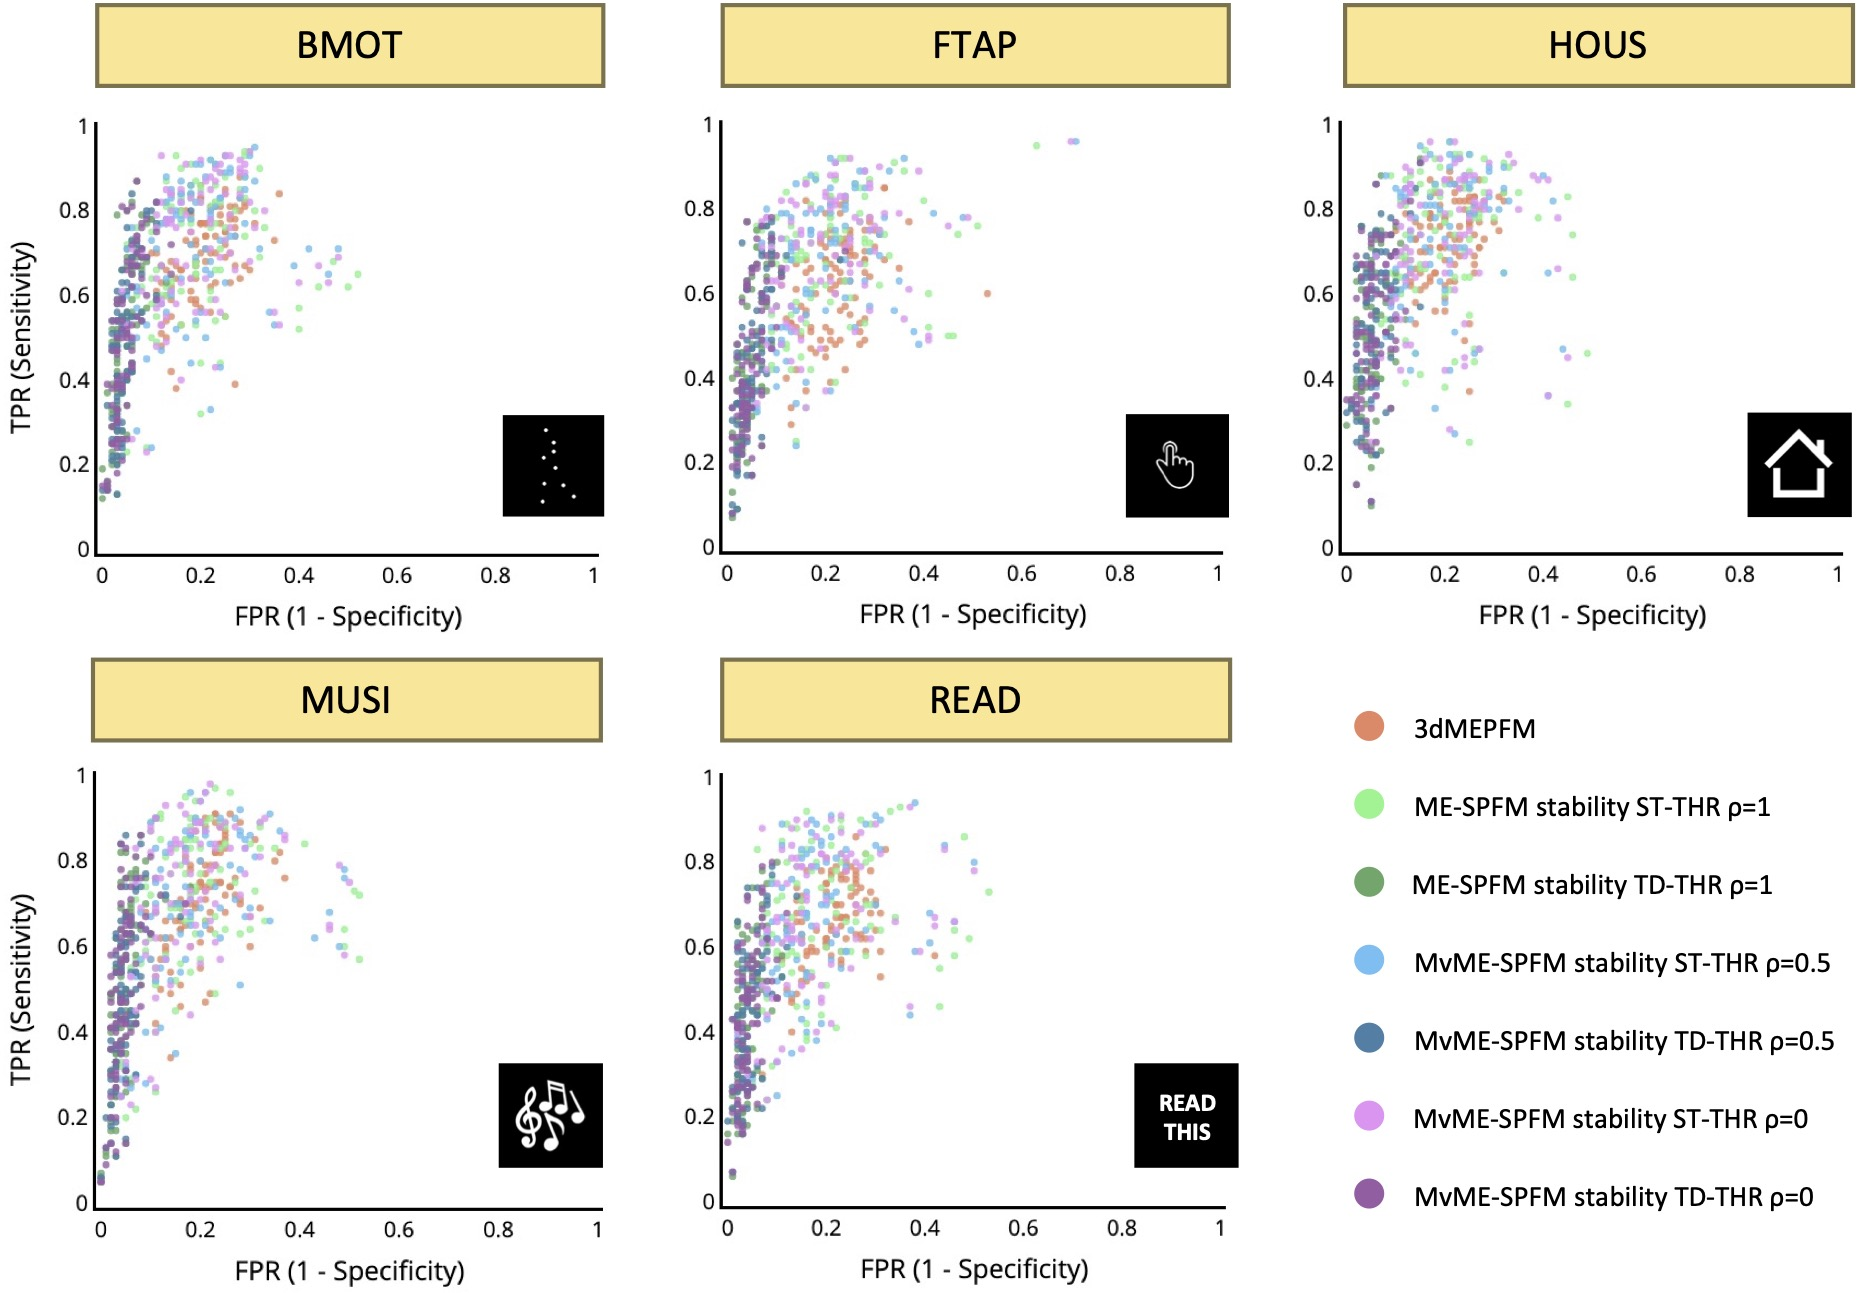
\includegraphics[width=0.8\textwidth]{figures/multivariate/roc.jpg}}
    \caption{Receiver operating characteristic (ROC) values with the sensitivity
    and specificity of each single trial's activation map for all conditions and
    the reference map obtained with a single-trial GLM. Different colors are
    used for the different analyses: the original ME-SPFM, and the novel
    MvME-SPFM approach using stability selection with the spatial regularization
    parameter set to $\rho=0.5$ and the two different thresholding methods:
    static (ST) and time-dependent (TD). In each analysis each dot represents a
    single trial, depicting all trials across all datasets, and the centroids
    across all the single trials are also shown for the three analyses.}
\label{fig:roc}
\end{figure}

These findings are further corroborated by the average activity maps across
trials, sessions and subjects for each condition in the task shown in
\cref{fig:group_avg}. The maps obtained with the novel MvME-SPFM technique with
stability selection and TD thresholding show a high resemblance to the average
of the single-trial GLM activation maps (3dDeconvolve with
independently-modulation (IM) option in AFNI, thresholded at $p<0.05$).
Interestingly, the MvME-SPFM approach seems to offer improved detection of
neuronal-related activity than the GLM approach for certain conditions, for
example, in the voxels of the left inferior frontal gyrus (i.e., Broca's region)
and left posterior superior temporal gyrus (i.e., Wernicke's region) for the
reading condition, where the GLM maps show a smaller cluster of activation.

\begin{figure}[ht!]
    \centerline{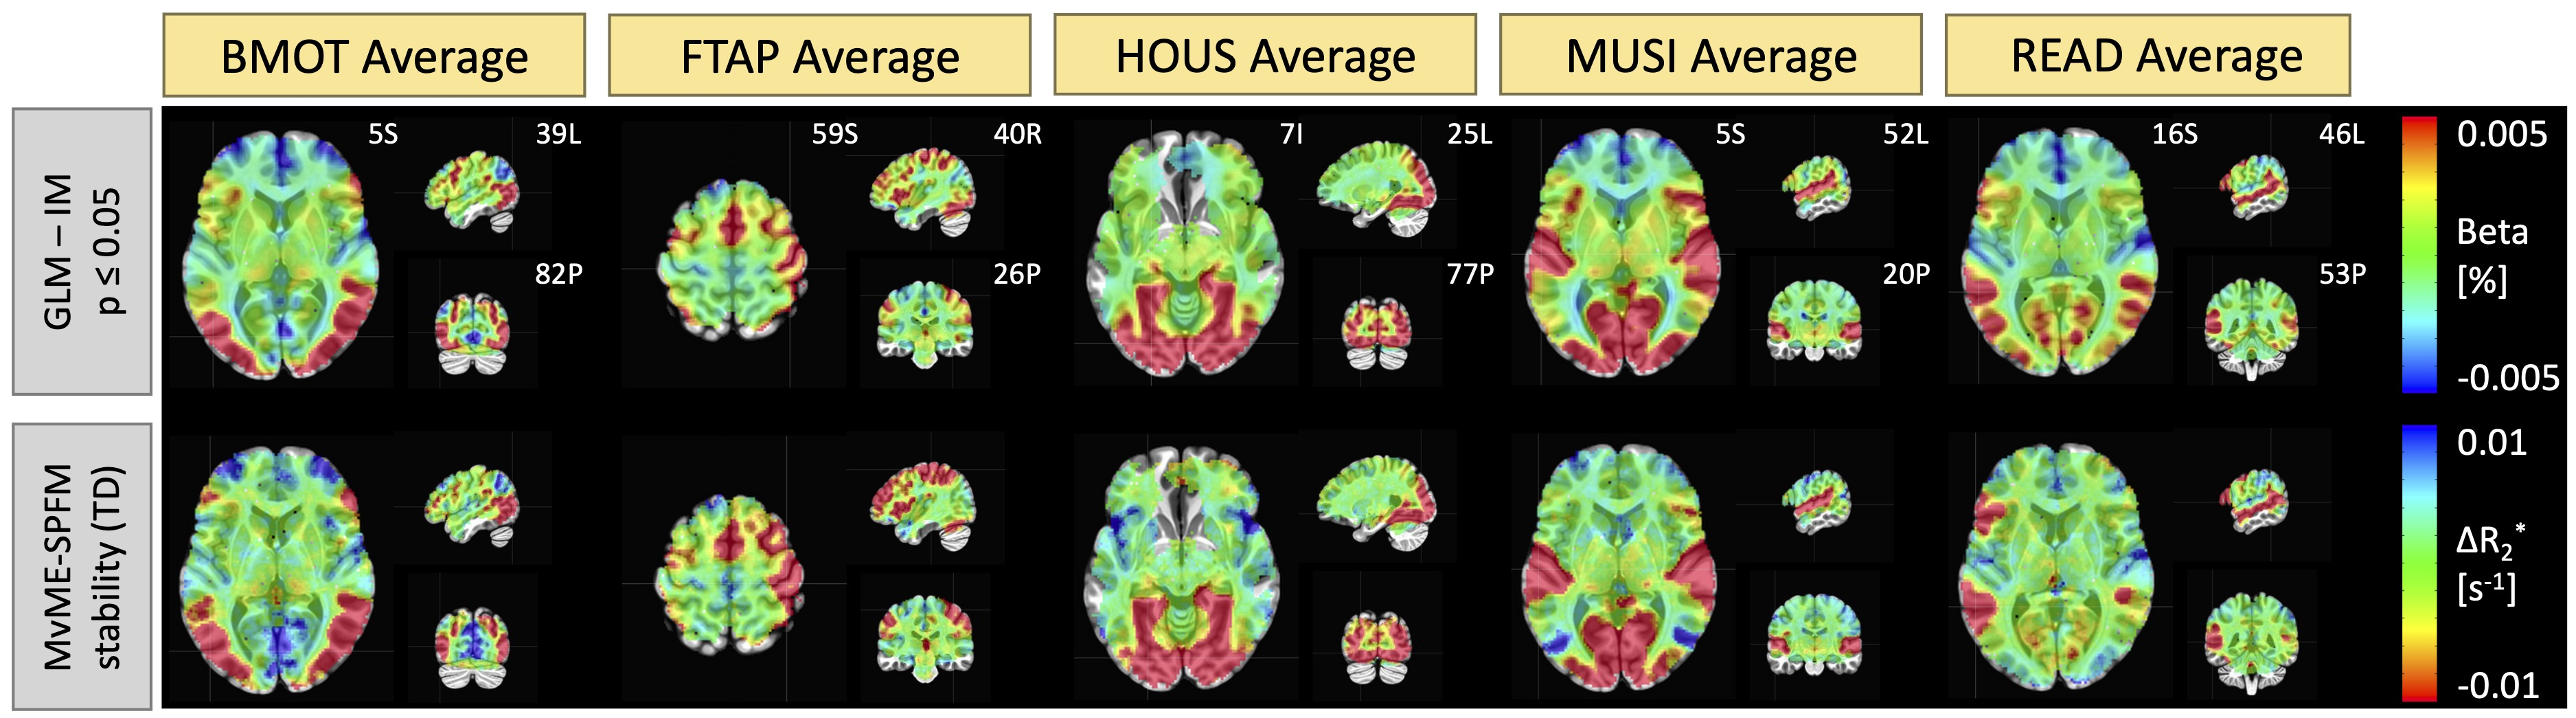
\includegraphics[width=\textwidth]{figures/multivariate/group_avg.jpg}}
    \caption{Average activity maps across trials, sessions and subjects for each
    condition in the task obtained with (top) a single-trial GLM analysis
    (independently modulated, IM) and the proposed MvME-SPFM algorithm with
    stability selection, $\rho=0.5$ and a time-dependent threshold (TD). }
\label{fig:group_avg}
\end{figure}

\cref{fig:hemolearn_comparison} shows the comparison with the HemoLearn
algorithm \citep{Cherkaoui2021Multivariatesemiblind}. Panels A and B illustrate
the difficulty of selecting a suitable number of components $K$ for Hemolearn
since the number of components giving the highest correlation to the
session-level GLM was different for each condition. The timecourses of the
estimated activity-inducing signal in C show that Hemolearn struggles to capture
the timings of the task in all conditions, while the MvME-SPFM technique with
stability selection and TD thresholding is able to capture the expected
activity-inducing signal with barely missing any of the events in the task.
These observations are also visible in the activity maps shown in D, where the
activity maps obtained with the MvME-SPFM technique with stability selection and
TD thresholding are comparable to those obtained with the GLM (see
\cref{fig:activity_maps}), while the maps of the Hemolearn components that had
the highest correlation with the session-level GLM maps do not show a clear
activity pattern related to the task.

\begin{figure}[ht!]
    \centerline{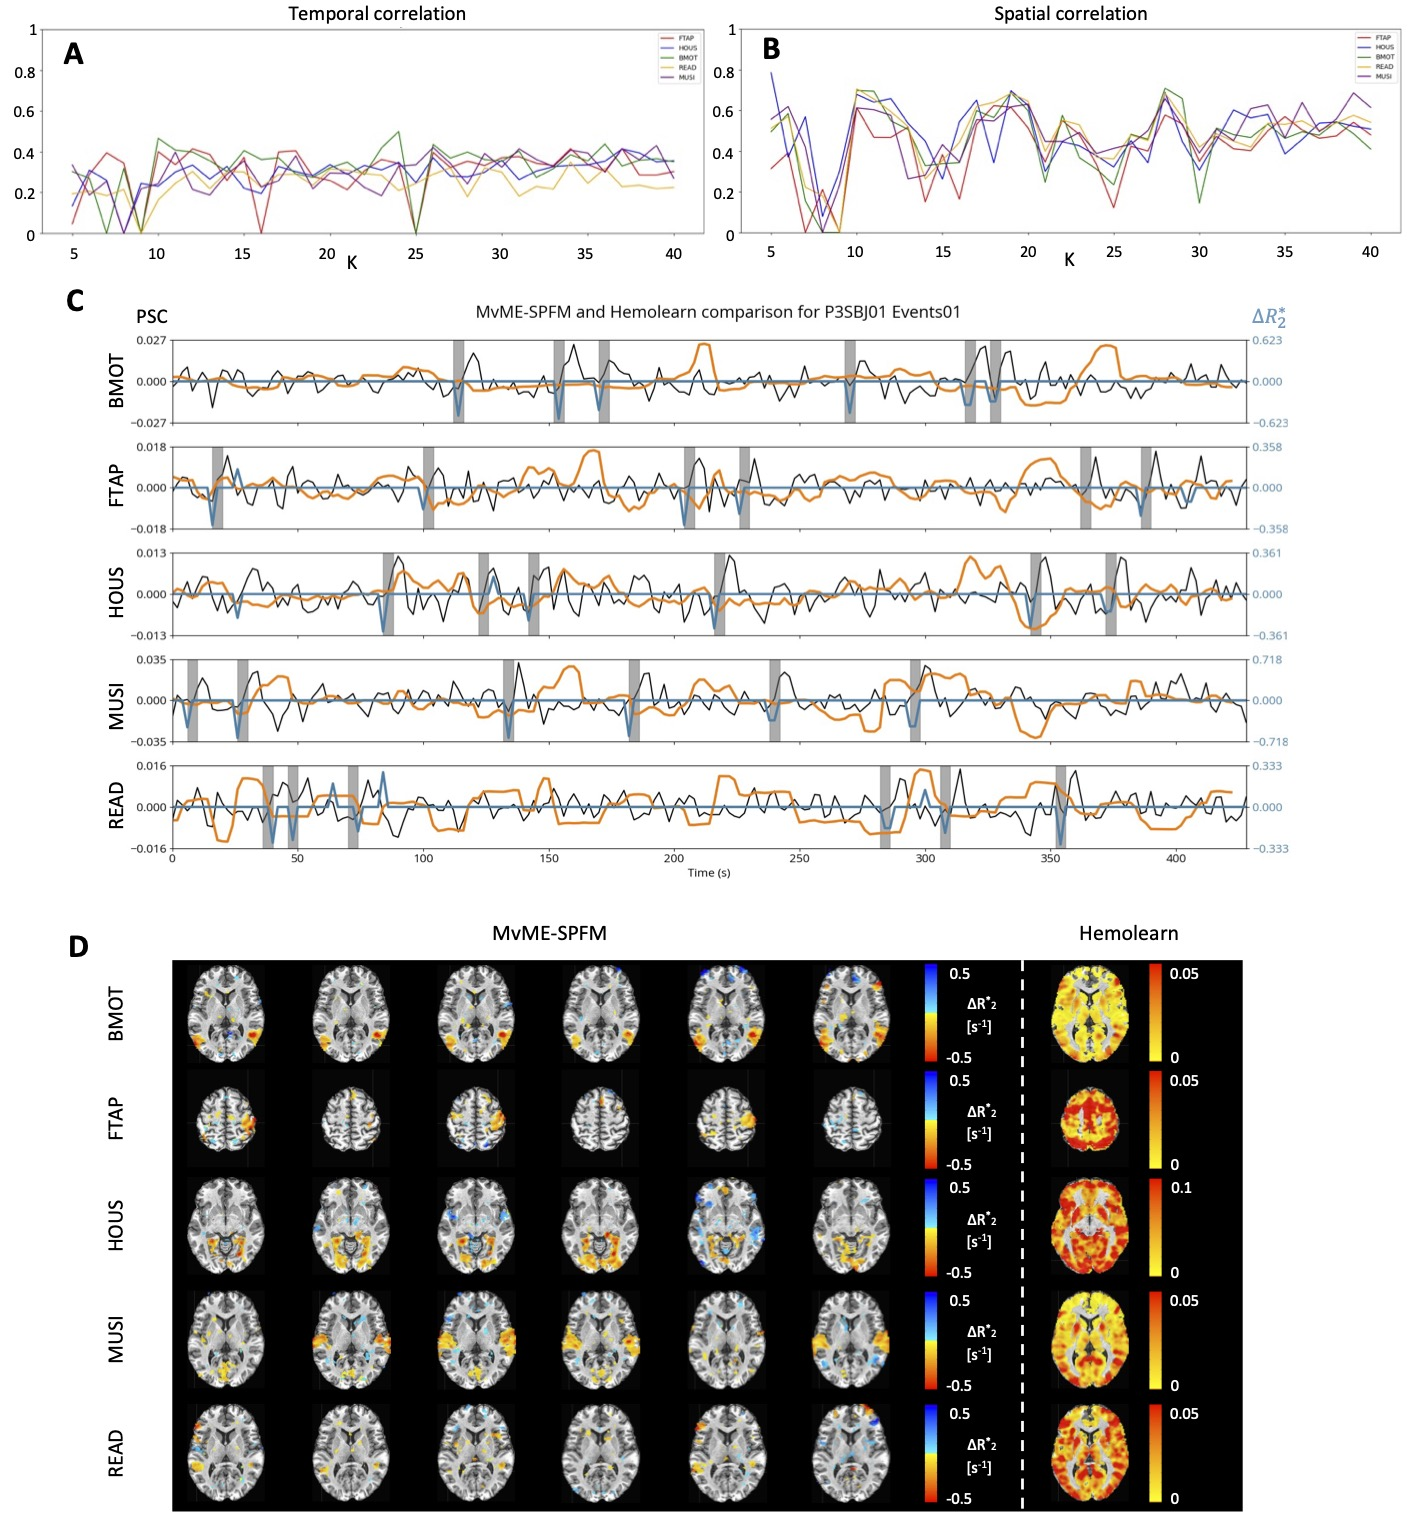
\includegraphics[width=\textwidth]{figures/multivariate/hemolearn_comparison.jpg}}
    \caption{Comparison of the activity maps obtained with the novel MvME-SPFM
    technique with stability selection, $\rho=0.5$ and a time-dependent
    threshold (TD) with Hemolearn. Session 1 of subject P3SBJ01 was used for
    this comparison. A and B show the highest correlation to the session-level
    GLM regressor and activity map respectively obtained by Hemolearn for each
    condition in the task (FTAP in red, HOUS in dark blue, BMOT in green, READ
    in yellow, and MUSI in purple) and the range of K components explored
    ($K=5\dots40$). C illustrates the timecourses of MvME-SPFM (blue, $\Delta
    R_2^*$) and Hemolearn-estimated (orange, percent signal change)
    activity-inducing signal in a representative voxel for each condition.}
\label{fig:hemolearn_comparison}
\end{figure}
\begin{figure}[ht!]
    \contcaption{The gray bars show the onset and duration of each trial within a
    condition, and the measured fMRI signal is shown in percent signal change
    (PSC) in black. D compares the trial-level activity maps estimated with
    MvME-SPFM with the Hemolearn activity map with the highest correlation with
    the session-level GLM map across the explored range of K components. Every
    row in C and D correspond to the different conditions in the task.}
\end{figure}

\section{Discussion and Conclusion}
\label{sec:multivariate_discussion}

The proposed whole-brain (i.e., multivariate) formulation for hemodynamic
deconvolution of multi-echo fMRI data with the use of stability selection
achieved a closer agreement with the activation maps obtained with a
single-trial GLM analysis than the original \acrshort*{mespfm} method
\citep{CaballeroGaudes2019deconvolutionalgorithmmulti} and other
state-of-the-art multivariate deconvolution method like Hemolearn
\citep{Cherkaoui2021Multivariatesemiblind}, while obviating the need to select
the temporal regularization parameter $\lambda$ (as shown in
\cref{fig:activity_maps} and \cref{fig:hemolearn_comparison}). 

Furthermore, this chapter demonstrated that the performance of the proposed
method was robust not only for the analysis of multi-echo data, but also when
analyzing single-echo data, as demonstrated in \cref{fig:hcp_motor}. In
addition, our results illustrated that the stability selection procedure also
offers robustness against the choice of the spatial regularization parameter
$\rho$, as the AUC maps for different selections of $\rho$ were practically
identical, as shown in \cref{fig:rho_comparison}. Hence, although stability
selection could be employed with a double selection of the regularization
parameters $\lambda$ and $\rho$, this can be avoided for computational reasons
with little influence in the results. In any case, extending the proposed
stability selection technique to other formulations of the hemodynamic
deconvolution problem, such as the voxel-wise (i.e., univariate) single-echo
\citep{Gaudes2013Paradigmfreemapping,Urunuela2020StabilityBasedSparse} described
in \cref{cha:synthesis_analysis} and \cref{cha:stability}, univariate multi-echo
\citep{CaballeroGaudes2019deconvolutionalgorithmmulti}, or low-rank and sparse
formulations
\citep{Urunuela2021LowRankSparse,Cherkaoui2021Multivariatesemiblind} described
in \cref{cha:low-rank}, is relatively straightforward.

One of the most interesting features of the proposed stability selection
procedure is the estimation of the area under the curve (AUC) measure, which
provides a new perspective for exploring fMRI data: a 4D movie with the
probability of each voxel and time point containing a neuronal-related event.
Therefore, the AUC time-series and maps provide complementary information to the
estimates of $\Delta R_2^*$, and serve as a reliability measure. Even though the
AUC measures were employed here to produce the final estimates of the
activity-inducing signal, they could also be exploited on their own. For
instance, they could be exploited to constrain functional connectivity analysis
\citep{Tagliazucchi2016VoxelWiseFunctional,Faskowitz2020Edgecentricfunctional}
to voxels and instants with a high probability of containing a neuronal-related
event. Furthermore, the stability selection and the AUC metric can also be
interpreted from a machine learning perspective, where the outputs from a
collection of lasso learners are combined with an ensemble regression approach.
Alternatively, the stability selection procedure could also be linked to
Bayesian approaches where the prior is given by the range of values of the
regularization term $\lambda$ and the total posterior probability of the
neuronal event is calculated as the integration of the stability paths, i.e.,
the AUC \citep[see discussion in][]{Meinshausen2010Stabilityselection}.

Although the estimation of the AUC eliminates the need to select the spatial and
temporal regularization parameters $\lambda$ and $\rho$, it requires the use of
a thresholding approach given the nature of the AUC measure, which cannot be
equal to zero by definition. This chapter adopted two data-driven thresholding
strategies, static (ST) and time-dependent (TD), based on the AUC values of a
region where no BOLD signal changes related to neuronal activity are assumed to
occur (e.g., deep white matter voxels). The use of a static AUC thresholding
approach yielded higher sensitivity than the original ME-SPFM method
\citep{CaballeroGaudes2019deconvolutionalgorithmmulti} while maintaining the
specificity as demonstrated in \cref{fig:roc}. Notably, this improvement was
seen in all trials with the exception of one outlier run, regardless of the
choice of the spatial regularization parameter $\rho$. Nevertheless, the use of
a time-dependent thresholding approach may be even justified by the increased
specificity and nearly perfect retrieval of the activity-inducing signal (row 3
in \cref{fig:dr2_time_series}) when motion- and respiration-related artifacts
are visible in the data (see arrows in \cref{fig:artifacts}). However, the
application of the time-dependent threshold may reduce sensitivity at the
single-trial level in some cases. Hence, the results shown in \cref{fig:roc}
encourage the use of the static thresholding approach as an exploratory step
before employing the time-dependent threshold. Other thresholding criteria could
involve the comparison of AUC values obtained from surrogate (null) data
\citep{Liegeois2021Interpretingnullmodels} with the AUC values obtained with the
original data.

Furthermore, the extension of the original ME-SPFM algorithm from a voxel-wise
to a whole-brain (i.e., multivariate) regularized problem paves the way for more
refined formulations that exploit the spatial characteristics and information
available in fMRI and complementary imaging data into the spatial regularization
term in order to improve the estimation of $\Delta R_2^*$. For instance, the
spatial regularization could be constrained within brain regions delineated by
commonly used parcellations (e.g., the Schaefer-Yeo atlas)
\citep{Karahanoglu2013TotalactivationfMRI} or within neighbouring gray matter
voxels \citep{Farouj2017Regularizedspatiotemporaldeconvolution}. Other
mixed-norm regularization terms could also be investigated in future work to
account for alternative models of spatially varying noise SNR, e.g., the
octagonal shrinkage and clustering algorithm for regression (OSCAR)
\citep{Gueddari2021CalibrationLessMulti}, which employs a $\ell_1$ plus a
pairwise $\ell_{\infty}$-norm between voxels instead of a global $\ell_2$-norm
to account for spatially varying SNR across voxels. Moreover, the multivariate
formulation could exploit complimentary multimodal information such as
structural connectivity from diffusion-based MRI data
\citep{Bolton2019StructurallyInformedDeconvolution}. In addition, the proposed
formulation can be easily adapted to model the changes in neuronal activity in
terms of its innovations, which can be more appropiate to capture sustained BOLD
events as described in \cref{cha:synthesis_analysis} (see also
\citep{Urunuela2023HemodynamicDeconvolutionDemystified}).

One limitation of the proposed MvME-SPFM technique is the assumption of a
particular shape of the hemodynamic response to construct the HRF matrix for
deconvolution in Eq.~\eqref{eq:multivariate_multi-echo_model}. The proposed
model does not account for the variability in the temporal characteristics of
the HRF across the brain, which originates from differences in stimulus
intensity and patterns, short inter-event intervals, or differences in the HRF
shape between resting-state and task-based paradigms
\citep{Yesilyurt2008DynamicsnonlinearitiesBOLD,Sadaghiani2009Neuralactivityinduced,Chen2021Investigatingmechanismsfast,Polimeni2021Imagingfasterneural}.
To resolve this issue, given that the performance of MvME-SPFM is not
time-locked to the trials, the current formulation could be extended to account
for variability in the onset of the activity-inducing signal, as well as to
introduce flexibility in the model, by employing multiple basis functions
\citep{Gaudes2012Structuredsparsedeconvolution}. Furthermore, our method could
be easily employed independently within parcels of any commonly-used atlases
with a pre-estimated, localized HRF. Finally, the computational demands involved
in the stability selection procedure, which solves the regularization problem in
Eq.~\eqref{eq:multivariate_multi-echo_inverse_problem} for a range of $\lambda$
values on a number of subsampled surrogate datasets, are higher than solving the
regularization path and finding an adequate solution via model selection
criteria as in ME-SPFM \citep{CaballeroGaudes2019deconvolutionalgorithmmulti}.
At the moment of writing, the method took approximately 10 hours to run on a
high-performance computing cluster parallelizing the stability selection
procedure so that each surrogate dataset was processed in a different core. 

\section{Code and data availability}
\label{sec:multivariate_github}
The code and materials used to generate the figures in this work can be found in
the following GitHub repository:
\url{https://github.com/eurunuela/MvMEPFM_figures}.

The Python package is available as part of \textit{splora} in the following
GitHub repository: \url{https://github.com/ParadigmFreeMapping/splora}.